\documentclass[]{article}
\usepackage{caption,subcaption,graphicx,float,url,amsmath,amssymb,tocloft}
\usepackage[hidelinks]{hyperref}
\usepackage[toc,acronym,nonumberlist]{glossaries}
\usepackage{titling}
\setacronymstyle{long-short}
\usepackage{glossaries-extra}
\graphicspath{{figs/}} 
\setlength{\cftsubsecindent}{0em}
\setlength{\cftsecnumwidth}{3em}
\setlength{\cftsubsecnumwidth}{3em}
\newcommand\numberthis{\addtocounter{equation}{1}\tag{\theequation}}
\pretitle{
	\begin{center}
		
\includegraphics[width=6cm]{KanjiLife}\\	
	}
	\posttitle{\end{center}}

%opening
\title{
	Notes from Origins of Life\\
	Week 6\\
	 Astrobiology \& General Theories of Life
}
\author{Simon Crase (compiler)\\simon@greenweaves.nz}

\makeglossaries
\renewcommand{\thesection}{6.\arabic{section}}

\loadglsentries{glossary-entries}

\renewcommand{\glstextformat}[1]{\textbf{\em #1}}

\begin{document}

\maketitle

\begin{abstract}
   These are my notes from the $6^{th}$ Week of the Santa Fe Institute Origins of Life Course\cite{sfi2020}. 
   The content and images contained herein are the intellectual property of the Santa Fe Institute, with the exception of any errors in transcription, which are my own.
   These notes are distributed in the hope that they will be useful,
   but without any warranty, and without even the implied warranty of
   merchantability or fitness for a particular purpose. All feedback is welcome,
   but I don't necessarily undertake to do anything with it.

\end{abstract}

\setcounter{tocdepth}{2}
\tableofcontents

\listoffigures

\section[Introduction]{Introduction--Chris Kempes}

Over the course of these lectures we have provided a range of tools and perspectives that would help us understand the origin of life on our own planet. These can be used to develop a general theory of life. Our ultimate goal is to provide a general theory of Life, one capable of uncovering the history we know about, but also bounding the possibilities for other types of life, and helping us recognize other forms of life. In this unit we'll discuss the search for life beyond Earth and how origins of life fits into this effort. We'll also discuss general evolutionary processes and abstract life. 

\section[Origins of Life and Astrobiology]{Origins of Life and Astrobiology-- Sara Imari Walker}

Hi I'm Sarah Walker, a professor at Arizona State University and an astrobiologist.
I study the origin of life.

And so one of the questions you might have as an astrobiologist is: why is origin of life so critical to the study of astrobiology?

Well, astrobiologists are really interested
in whether or not we can identify a
living world so if we can identify
life on another planet.
We want to discover aliens and
ultimately, the question is whether we'll
be able to distinguish planets that have
life from plants that don't have life. So
in our own solar system, we can actually send robotic missions to other planets to look for life on the surface of those worlds but we're thinking about exoplanets and planets and distant solar systems all that we're going to get is a little bit of data about the entire planet.

As astrobiologists we are interested in thinking about life not only at the scale of individual organisms, but also at the scale of entire planets. 
And so just to talk about the magnitude of the problem a lot of people want to talk about looking at life in kind of new ways and maybe trying to use insights from different aspects of known fields of science to try to understand how we identify life.
Figure \ref{fig:Jupiter:Tellus} shows two worlds that are probably familiar to everyone, Jupiter and Earth; we know one of these planets is inhabited and the other isn't.
\begin{figure}[H]
	\caption[What makes worlds with life different?]{What makes worlds with life different? Not just non-equilibrium structures.}\label{fig:Jupiter:Tellus}
	\begin{subfigure}[b]{0.44\textwidth}
		\caption{Jupiter has its Great Red Spot}\label{fig:Jupiter}
		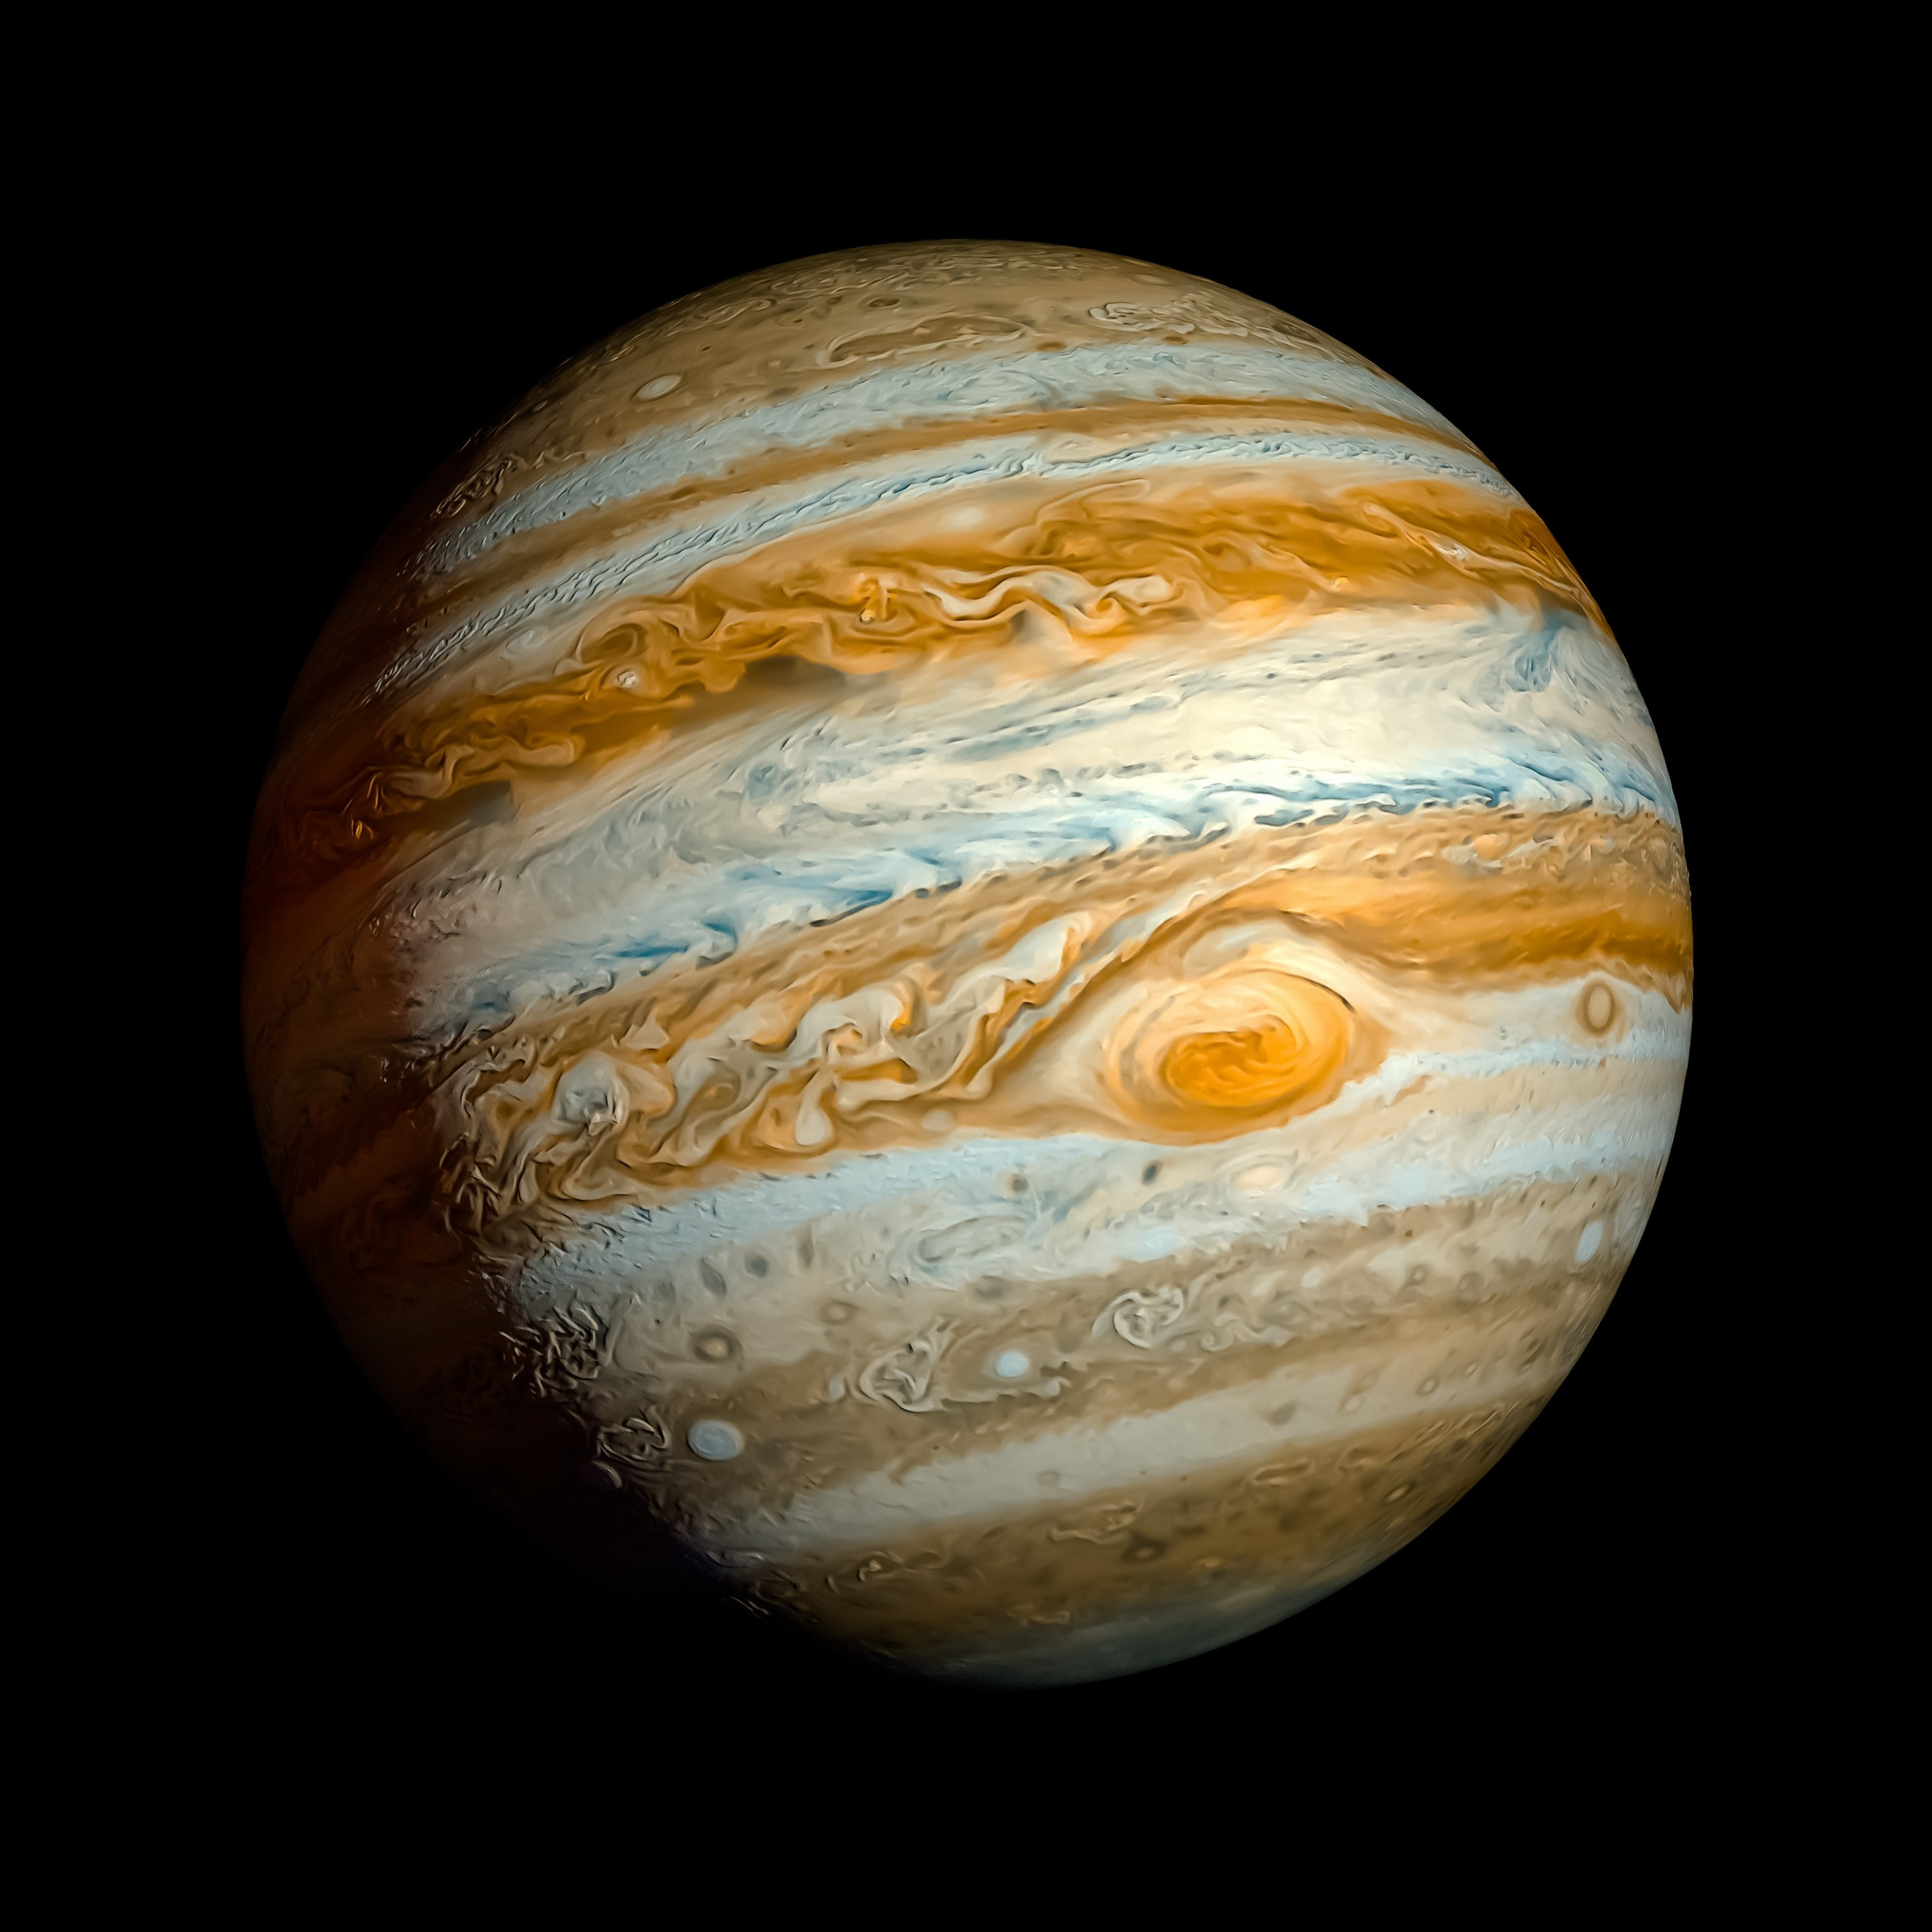
\includegraphics[width=\textwidth]{Jupiter}
	\end{subfigure}
	\;\;\;
	\begin{subfigure}[b]{0.5\textwidth}
		\caption{Earth at night, showing cities.}\label{fig:Earth}
		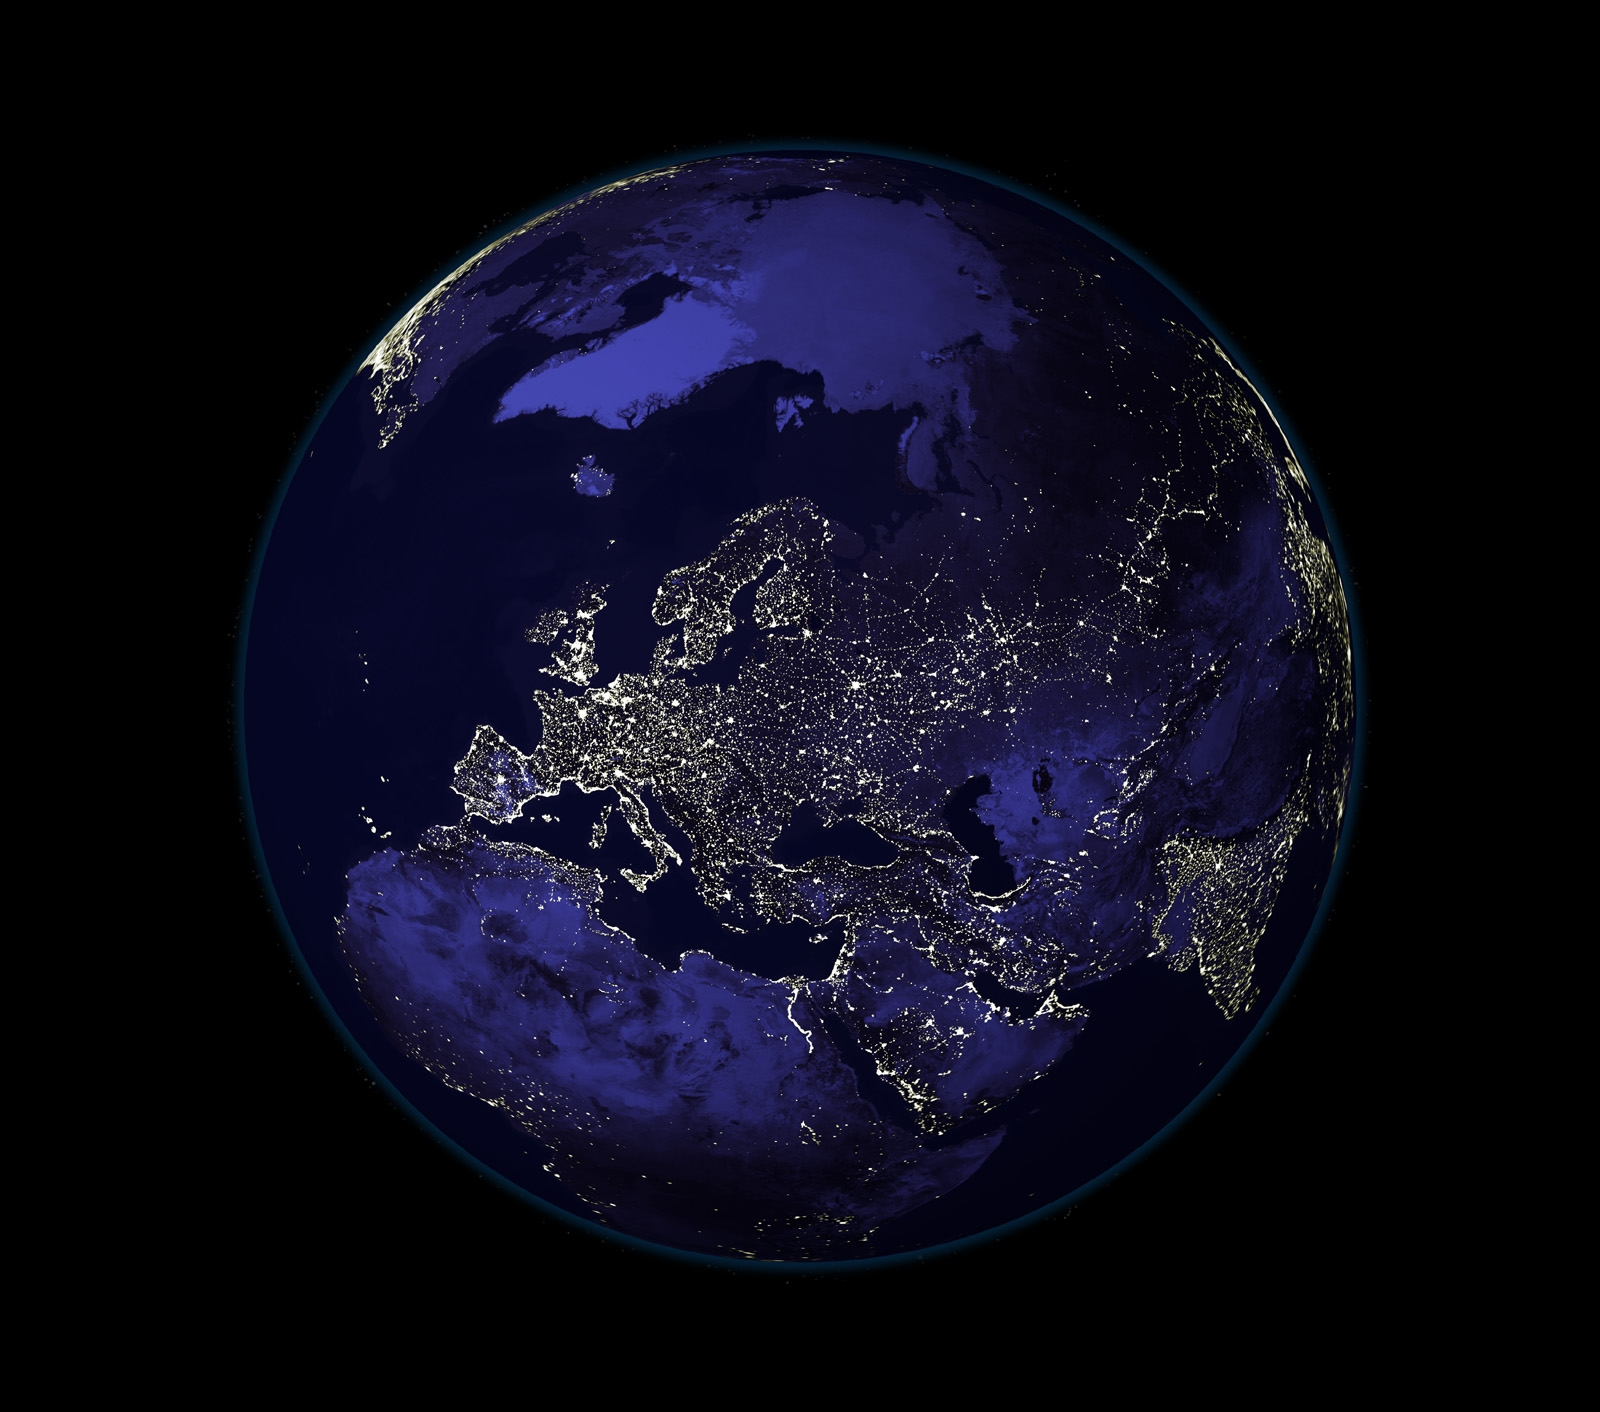
\includegraphics[width=\textwidth]{Tellus}
	\end{subfigure}
\end{figure}

The inhabited world is obviously our
very own earth, and we can see living
structures on its surface what we see
here is cities at night. When we're
thinking about how to think about the
problem of distinguishing the living
process on Earth from the nonliving
process on Jupiter, it's clear that both
have non-equilibrium structures on
their surfaces. So Jupiter for example
has this great red spot and as I
mentioned, earth has cities. So when we
want to talk about defining the
properties of those planets that are
associated with life, it's not just about
this disequilibra. Clearly cities are
fundamentally different than the great
red spot of Jupiter even though they're
both non-equilibrium structures. So we
have to move a little bit further and
understand the origins of the processes
that led to structure
on the surface of our planet that are
associated with life, and the root of
that question is really to understand
what's the probability of life emerging
on a planet--Figure \ref{fig:P:Life} and how can we actually
understand that as a planetary scale
process. 

\begin{figure}[H]
	\caption[Rate of abiogenesis in a prebiotic environment]{Rate of abiogenesis in a prebiotic environment as a function of its physical and chemical conditions}\label{fig:P:Life}
	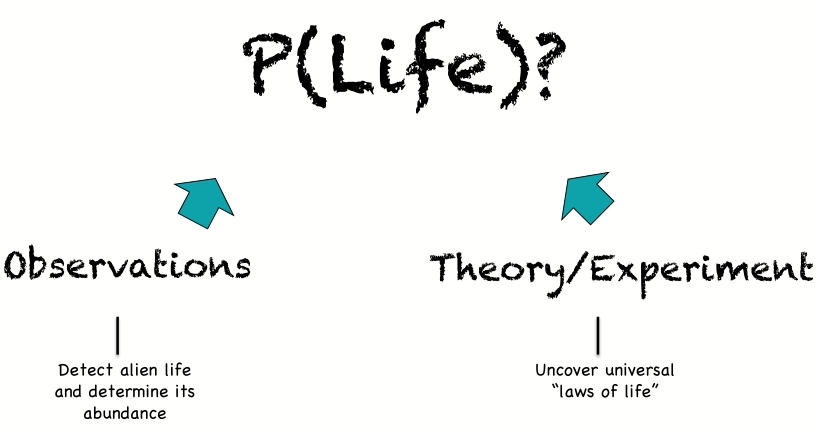
\includegraphics[width=0.9\textwidth]{P_Life}
\end{figure}


There's really two ways of
constraining the likelihood of life
emerging on a planet. We don't
think that Jupiter is a living planet. Obviously
based on our observations of Jupiter, it
could be that it might satisfy some
definition of life down the road if we
actually come up with a theory for life
and Jupiter satisfies that theory but
right now we don't think Jupiter's alive.

And so we need some observations of
other living world to constrain the
probability of life right now earth is
the only example we know and so to do
that we actually have to detect alien
life and determine its abundance. And so
this is the way you usually people think
about astrobiology is actually looking
at other worlds trying to identify if
there's aliens on those worlds and then
maybe we would actually be able to
constrain the probability that a planet
like Earth is going to emerge life on
its surface and a planet like Jupiter is
not. 

But we can also think about theory
and experiment to constrain the
probability for life. And from this view
the idea is really to try to uncover
what are the universal principles of
life that might actually allow us to
build predictive models for the
circumstances under which life should
emerge. So, we would have some a priori
theory that would enable us to predict $P(life)$--
the probability of life emerging.
And  that theory should be
able to account for the differences in Figure \ref{fig:Jupiter:Tellus} that
it's not just a non-equilibrium process
on the surface of a planet but in the
case of formation of cities or forests
or any of the kind of rich structure
that we see on earth that's a product of
biology that the theory would be able to
explain what those things are and be
able to predict what kinds of other
examples of life we might be able to see
on other planets and their likelihood.

But really what we're talking about in
order to constrain the probability of
life is not just to think about the
probability of forests or cities on the
surface of planets as opposed to the
probability of great red spots or other
kinds of dissipative structures that
aren't alive. What we really want is to
understand what's the likelihood of life
even emerging on that planet.
So we really need to be able to solve
the origin of life problem in order to do
astrobiology effectively and constrain
the likelihood of life in the universe.

And so in order to do that, we have to
come up with better theories for origins
of life and be able to understand how
life emerges. And so one of the ways I
like to think about it is really that
we're looking for new principles that
would explain life not just on earth but
life on other planets and I really love
this quote from David Deutsch which I
think articulates very nicely the kind
of processes that are happening on
planets that we really need to be able
to understand in order to understand
life. 

\begin{quotation}
	Base metals can be transmuted into gold by stars, and by intelligent beings who understand the processes that power stars, and by nothing else in the universe--David Deutsch\cite{deutsch2011beginning}.
\end{quotation}

We have a physics that explains things like stars or the physics of Jupiter and why Jupiter has a great storm on the surface of the planet at the great red spot.
But we don't have a physics that explains the evolution of a planet like our own, how life emerges on that planet, or how it evolves over time to lead to the kind of diversity of structures that we have on the surface of our planet today, like cities and
thinking human beings.

\begin{figure}[H]
	\begin{center}
		\caption[We don't have a physics that explains the evolution of our planet]{We don't have a physics that explains the evolution of a planet like our own}\label{fig:tellus}
		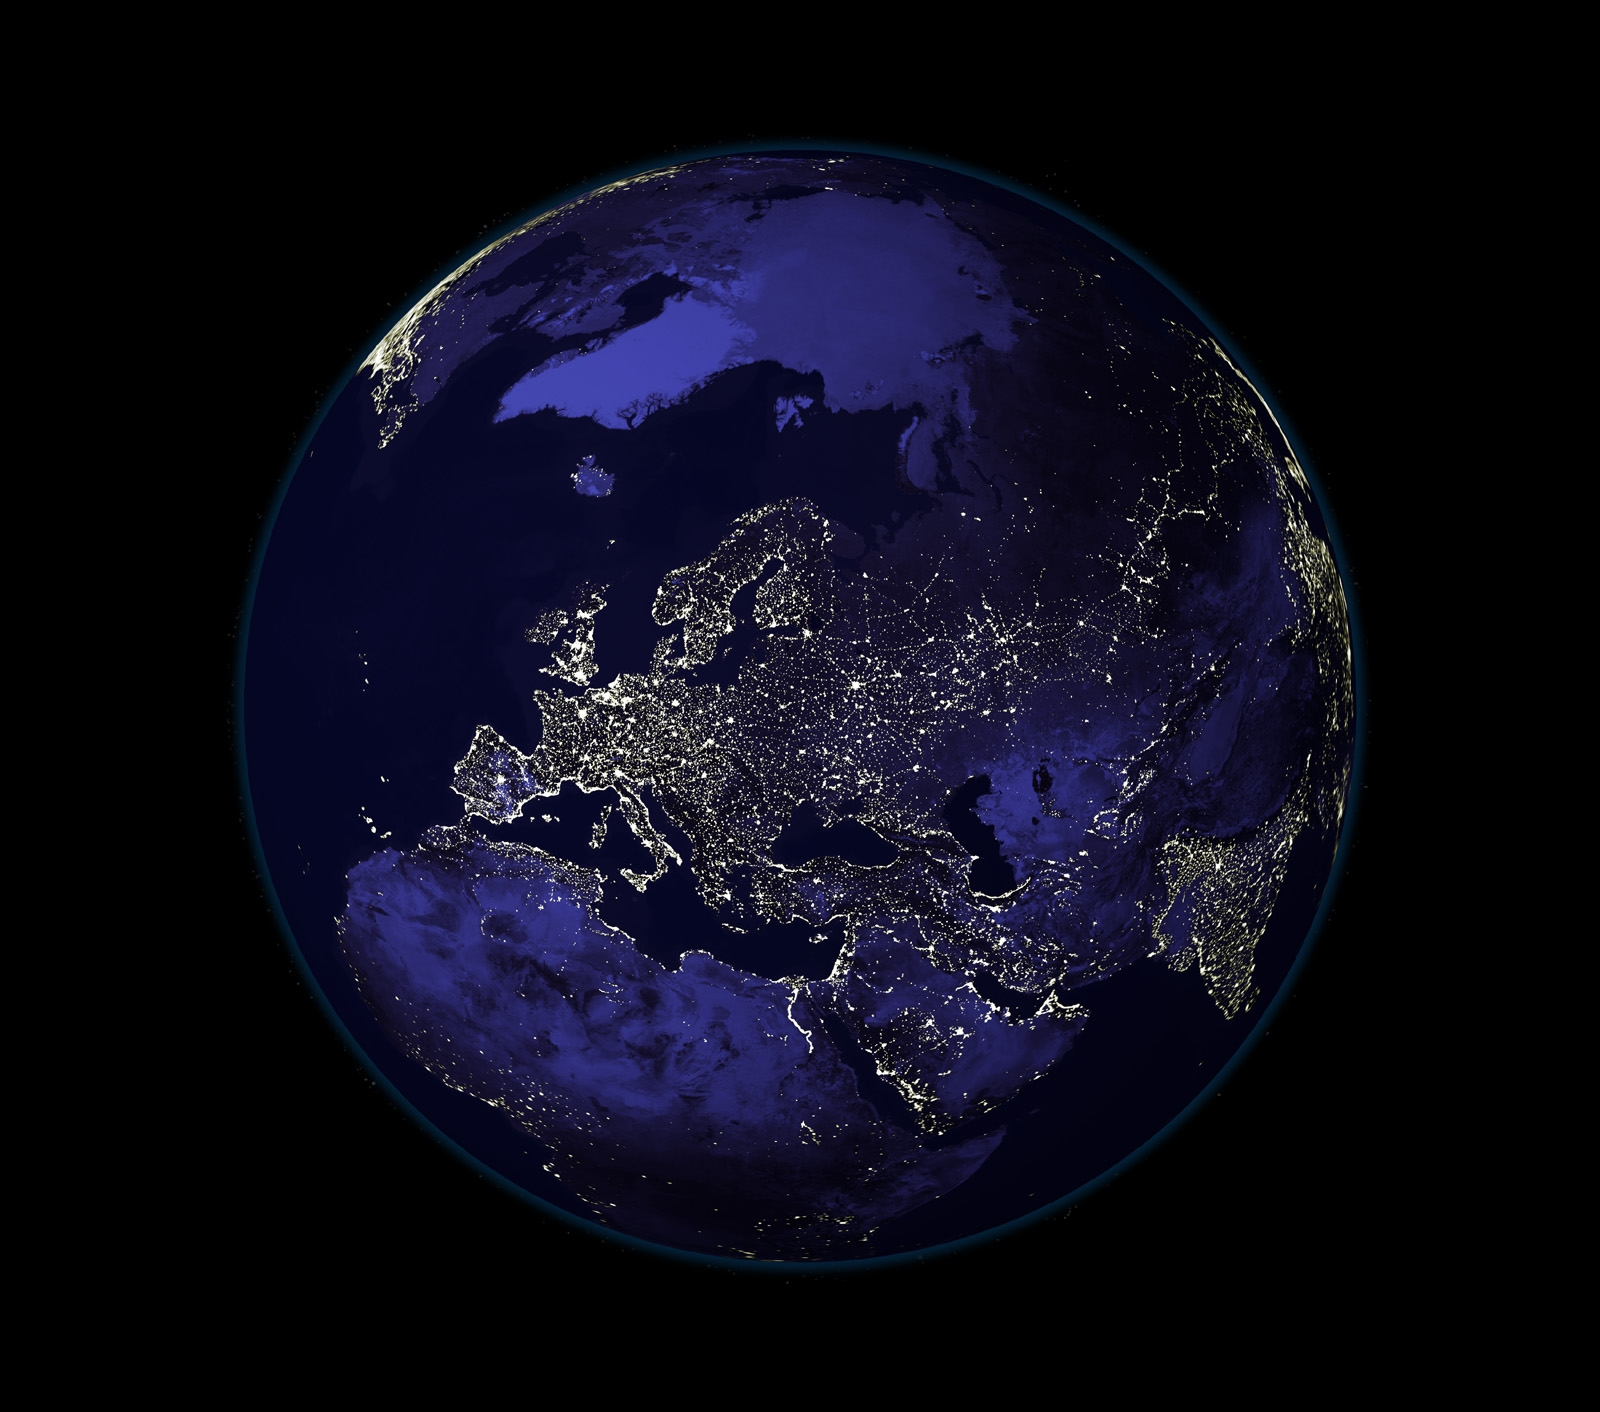
\includegraphics[width=0.5\textwidth]{Tellus}
	\end{center}
\end{figure}

The origin of life problem is really a problem of how that entire process of life gets started in the first place and it's ultimately critically important to the field of astrobiology that we understand that process because we want to know on how many worlds that occurs.


\section{Exoplanets}

\subsection[The Habitable Zone]{The Habitable Zone--Elizabeth Tasker}


This lecture takes us away
from our own planet
to look at what we currently know about
planets orbiting around other stars.
Before the early 1990s, the only planets
we knew for sure that existed
were the worlds that orbited
around our own Sun,
but as our instruments
became sensitive enough to spot
the dim whisper of a planet
around other stars in our galaxy,
we discovered our planetary system
was one of multitudes--Figure \ref{fig:exoplants}.


\begin{figure}[H]
	\caption{Exoplanets by discovery technique}\label{fig:exoplants}
	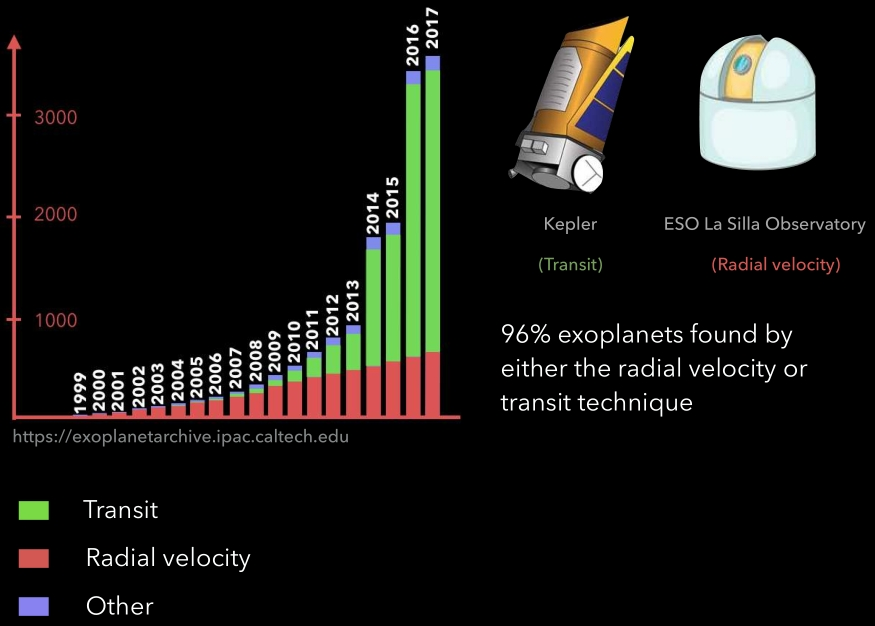
\includegraphics[width=0.9\textwidth]{Exoplanets}
\end{figure}

We now know of thousands of
extrasolar planets or exoplanets -
planets that orbit stars
other than our Sun.
This results in an obvious question:
could any of these newly discovered
worlds be habitable?

\begin{figure}[H]
	\caption{Could any of these newly discovered
		worlds be habitable?}\label{fig:could-any-be-habitable}
	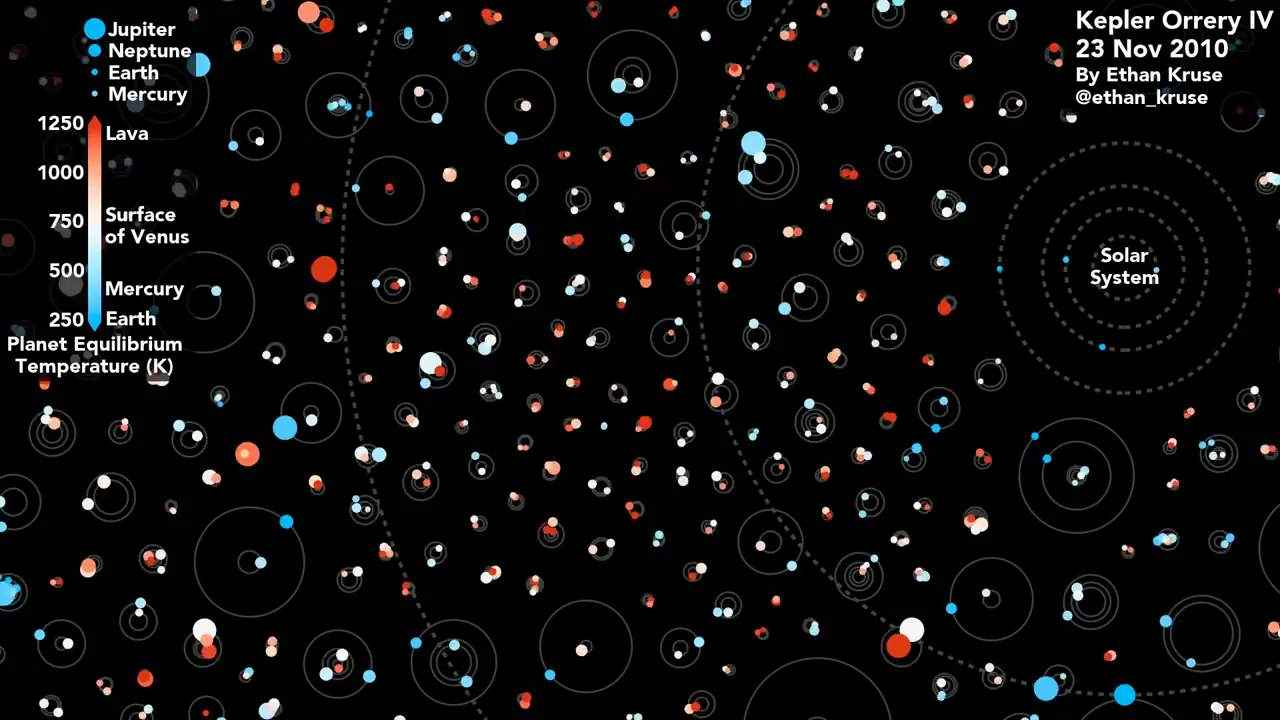
\includegraphics[width=\textwidth]{could-any-be-habitable}
\end{figure}
The problem with that question is,
while we have discovered many worlds,
we actually know very little
about each planet.
The majority of planets
we have discovered so far
have been found by one
of two techniques--Figure \ref{fig:exoplants}:
\begin{enumerate}
	\item the radial velocity technique used by ground-based telescopes, such as the ESO Observatory in Chile----Figure \ref{fig:radio-velocity-technique0};
	\item the transit technique used by instruments such as the Kepler space telescope and its successor - TESS--Figure \ref{fig:transit}.
\end{enumerate}

\begin{figure}[H]
	\caption[The radial velocity technique]{The radial velocity technique, sometimes known as the "Doppler wobble," detects a planet via the tiny wobble it excites in the star. While we normally think of the star as stationary and the planet in orbit, in truth, both the star and planet orbit their common center of mass--Figure \ref{fig:radio-velocity-technique}. As a star is so much bigger than the planet, this center of mass lies very close to the star's own center, causing its orbit to be just a tiny wobble in comparison to the planet's wide circuit. This wobble causes the star to move periodically slightly further away and then closer to the Earth. As the star moves slightly from the Earth, its light waves stretch out and redden slightly--Figure \ref{fig:radio-velocity-technique1}. Conversely, as a star moves back towards us, the light waves compress and become bluer. This regular shift from red to blue is what astronomers can measure to detect a planet--Figure \ref{fig:radio-velocity-technique2}.}\label{fig:radio-velocity-technique0}
	\begin{subfigure}[t]{0.3\textwidth}
		\caption{The star and planet orbit their common center of mass}\label{fig:radio-velocity-technique}
		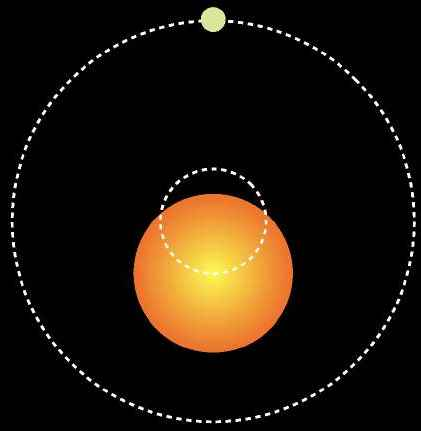
\includegraphics[width=\textwidth]{radio-velocity-technique}
	\end{subfigure}
	\;\;\;
	\begin{subfigure}[t]{0.3\textwidth}
		\caption{As the star moves slightly from the Earth, its light waves stretch out and redden slightly}\label{fig:radio-velocity-technique1}
		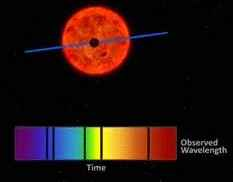
\includegraphics[width=\textwidth]{radio-velocity-technique1}
	\end{subfigure}
	\;\;\;
	\begin{subfigure}[t]{0.3\textwidth}
		\caption{This regular shift from red to blue is what astronomers can measure to detect a planet}\label{fig:radio-velocity-technique2}
		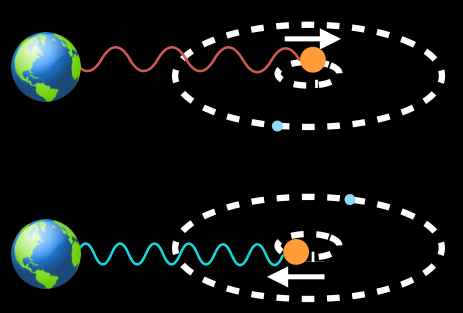
\includegraphics[width=\textwidth]{radio-velocity-technique2}
	\end{subfigure}
\end{figure}

\begin{figure}[H]
	\begin{center}
		\caption[The transit technique]{The second main method for planet detection is the transit technique. Here, a slight dip in the star's brightness is detected as the planet passes in front of the star as seen from Earth.}\label{fig:transit}
		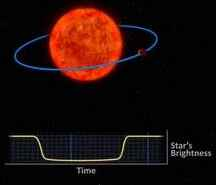
\includegraphics[width=0.5\textwidth]{transit}
	\end{center}
\end{figure}

These two methods give you
just two properties about the planet--Figure \ref{fig:planet-properties}.
The transit technique gives you
an estimate of the planet's radius
while the radial velocity technique
tells you about the planet's
minimum mass.
This may be significantly less
than the true mass of the planets
as the radial velocity technique
only measures the wobble of the star
directly towards the Earth.
If the planet's orbit is tilted
with respect to us,
then part of the star's motion
will be directed away from us.
We won't measure this and so
underestimate the planet mass.

\begin{figure}[H]
	\begin{center}
		\caption{These two methods give you
		just two properties about the planet}\label{fig:planet-properties}
		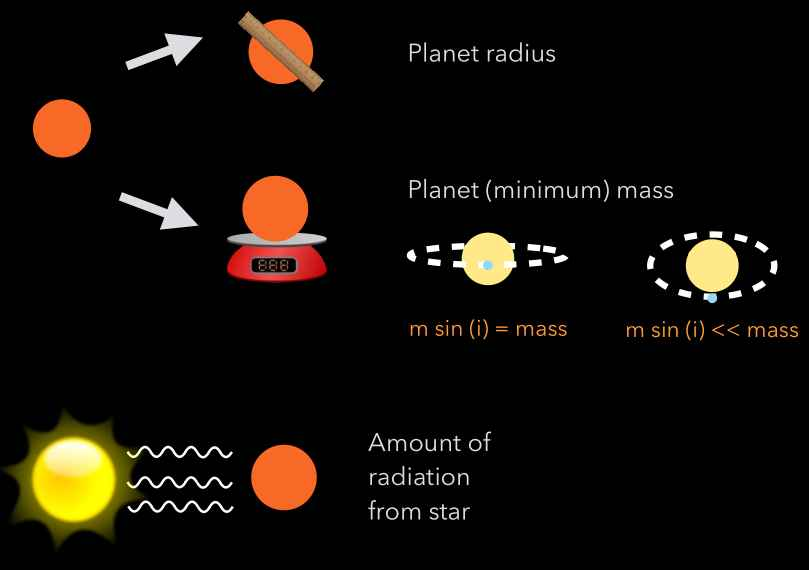
\includegraphics[width=0.8\textwidth]{planet-properties}
	\end{center}
\end{figure}
Both techniques also tell you about
the amount of radiation
the planet receives from the star.
But, this can be very different
from the surface temperature
as it does not allow for
the heat trapping effects
of the different atmospheric gases.

The challenge we're trying to determine -
if a plant is habitable -
is therefore that we can only measure
two or three properties
and none of these actually tell us
what it's like on the planet surface.
This will change as
the next generation of telescopes
will be able to detect light that passes
through the planet's atmosphere.
Different molecules in the atmosphere
absorb different wavelengths of light,
providing a fingerprint
of missing wavelengths
that indicate atmospheric composition -
our first hint at what is happening
on the planet's surface.

But, this brings us to a new problem:
such atmospheric spectroscopy
for rocky, temperate planets
is time-consuming and difficult.
We therefore need a way
of selecting planets
most likely to reveal interesting results.
But how do we select planets
best suited for habitability
without knowing any surface properties?

Let's think about what we want to find.
It's going to be easiest
to recognize Earth-like life,
that is, water and
carbon-based chemistry.
Also, this needs to be detectable,
which means the water needs to be
on the surface of the planet,
not a subsurface system like Europa.

Based on this, we can ask the question:
how much insolation
does an Earth-like planet need?
The answer to this is
a \emph{Classical Habitable Zone}--Figure \ref{fig:classical:habitable:zone}.

\begin{figure}[H]
	\caption{Classical Habitable Zone}\label{fig:classical:habitable:zone}
	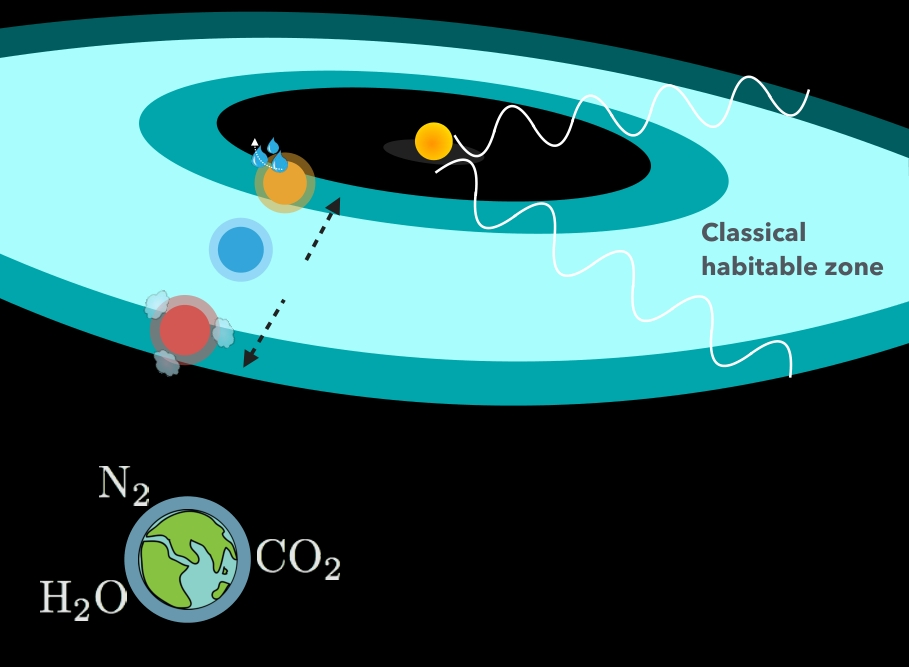
\includegraphics[width=\textwidth]{ClassicalHabitableZone}
\end{figure}

The Classical Habitable Zone
is where an Earth-like planet,
that is, a planet with
our surface pressure,
atmospheric gases
and geological processes
can support water on the surface.
Often, in exoplanet literature,
this is simply referred to
as the "habitable zone"
as we don't yet know about planets
other than the Earth
that can support life.
At the inner edge of the habitable zone,
it is too warm for surface water
on the Earth and it evaporates.
At the outer edge, carbon dioxide
condenses into clouds
and is no longer able to provide
the thermal insulation
of a greenhouse gas -
so the planet freezes.
Climate models predict that
the habitable zone should stretch
between 0.99 au and 1.67 au
where 1 au is the average distance
of the Earth from the Sun.
Our planet, therefore,
sits right on the inner edge.

A slight extension to this is known as
the "optimistic habitable zone,"
which can broaden these limits
based on the idea
that Venus and Mars probably have
supported surface water in their past--Figure \ref{fig:optimistic:habitable:zone}.

\begin{figure}[H]
	\caption[Optimistic Habitable Zone]{Optimistic Habitable Zone\cite{kasting1993habitable,kopparapu2013habitable}}\label{fig:optimistic:habitable:zone}
	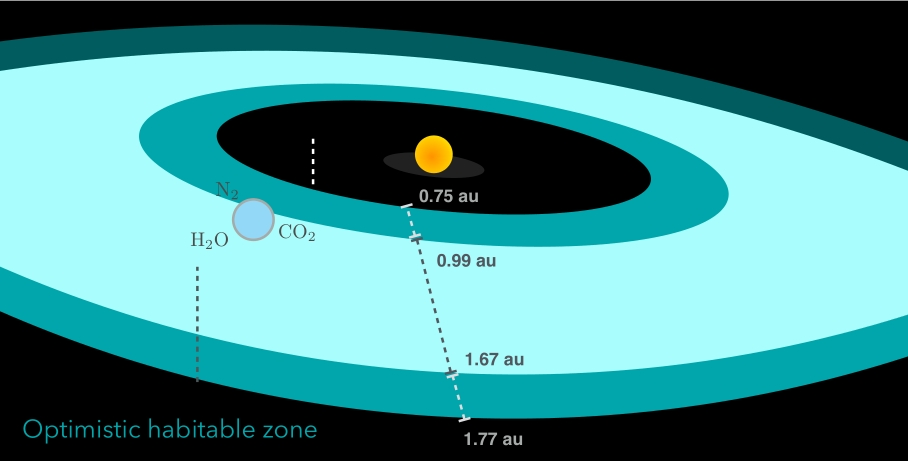
\includegraphics[width=0.9\textwidth]{OptimisticHabitableZone.jpg}
\end{figure}

So, an earth-like planet
could have a period of habitability
just outside the habitable zone edges.
The edges of the classical habitable zone
are only calculated for the Earth.
This is easily demonstrated as,
while Venus sits outside
the habitable zone,
both the Moon and Mars orbit within it
but neither are Earth-like enough
to support liquid water in this region.
Different planets might have different
habitable zones at different locations,
or they may not have
a habitable zone at all.

Of the planets we found so far orbiting
in the classical habitable zone,
almost 15 times as many
are large enough
to likely have thick,
Neptune-like atmospheres
compared to planets that might be rocky.
We have discovered planets
that are the right size to be rocky
and orbit entirely within
the habitable zone--Figure \ref{fig:are:these:earthlike}.
Are these Earth-like enough
to support liquid water in this region?



We don't know.
They may have very different
atmospheric gases
or geology that makes
surface water impossible.
The only thing we can say is that
if another habitable,
Earth-like planet is out there,
it would be in the habitable zone,
but being in the habitable zone
does not mean you're
Earth-like enough for life.

\begin{figure}[H]
	\caption{Are these exoplanets Earth-like?}\label{fig:are:these:earthlike}
	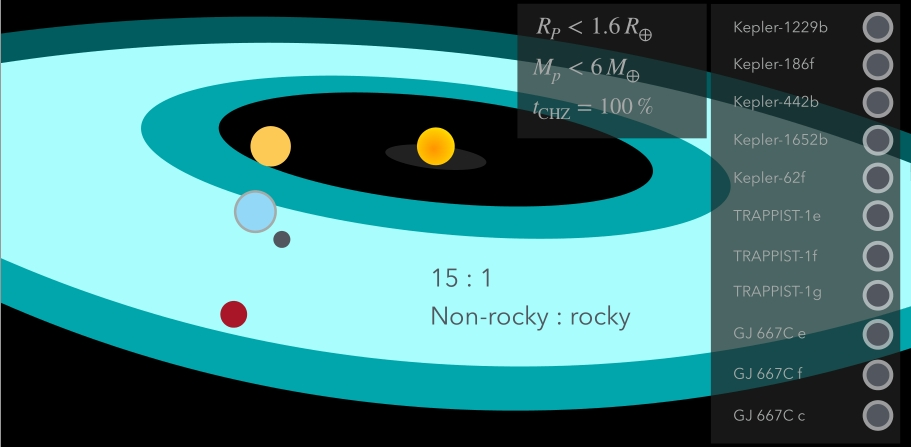
\includegraphics[width=0.9\textwidth]{AreTheseEarthlike}
\end{figure}

So, in conclusion,\begin{itemize}
	\item  we've discovered thousands of exoplanets, many of which are similar in size to the Earth. 
	\item But, at the moment, we have no way of knowing what their surfaces are like. Note, in particular, that the Earth and Venus are both very similar in size--so, they are both Earth-sized planets.
	\item Our next generation of telescopes will be able to detect the atmosphere of these worlds and tell us something about their surfaces for the first time.
	
	\item The habitable zone is a useful concept for selecting planets for these new telescopes but it offers no guarantee that a planet is actually habitable.
\end{itemize}

If you'd like to try playing with a simple climate model of an Earth-like planet, you can head over to "earthlike.world" or the associated Twitter feed. This website lets you see how different a planet might be from our own world today, even if it did have the same geological cycles as our own.

The NASA NExSS "Many Worlds" blog covers the latest news for exoplanets
and many origin of life stories.
There's also a more technical overview of the search for biosignatures in a paper led by Yuka Fujii, published in "Astrobiology" last year.
These are the references that were mentioned during the lecture.

See also \cite{fujii2018exoplanet,villanueva2015unique}.

\subsection[Exoplanet Atmospheric Characterization]{Exoplanet Atmospheric Characterization--Yuka Fujii}

Astronomers have discovered
thousands of extrasolar planets
or exoplanets.
Is any of them inhabited like the Earth?
How can we search for it?
In this lecture, I will talk about
the techniques to study exoplanet
atmospheres and possibly surfaces,
which is an essential step towards
finding life on exoplanets.
Detection of exoplanets typically
comes with two properties:
the size and the orbit,
including the distance from the host star--Figure \ref{fig:discovered:exoplanets}.

\begin{figure}[H]
	\caption{Discovered Exoplanets}\label{fig:discovered:exoplanets}
	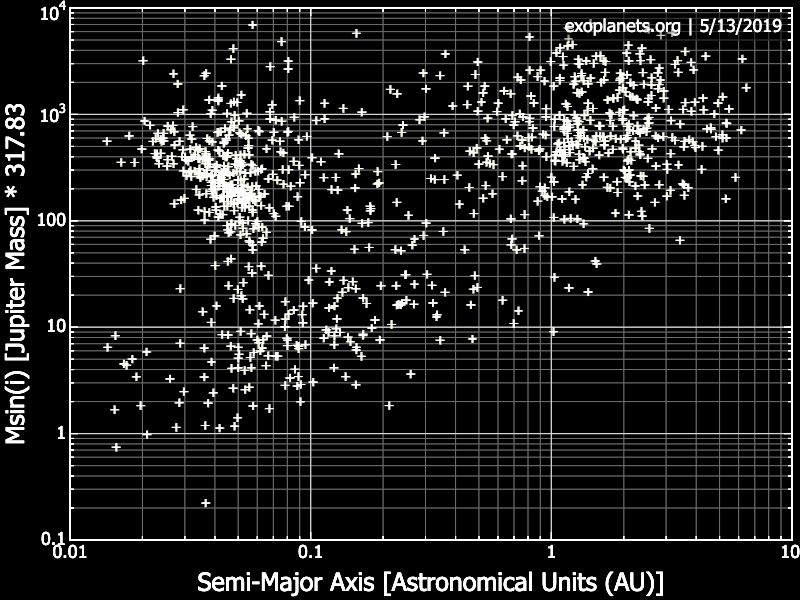
\includegraphics[width=0.9\textwidth]{ExoplanetCharacteristics}
\end{figure} 


For evaluating their potential for life,
we definitely need to get
more information.
But, how?
It has to be reminded that
exoplanets are light-years away.
This means that it's not realistic
to actually visit there
and it's not possible either
to get the spatially resolved images,
unlike the case of solar system planets.
They are just point sources
and we have to rely on remote
observations of these faint dots.
But, observations of these faint dots,
if possible at all,
can in principle give us hints
about the nature of the planets.
For example,
if you observe an Earth Twin--Figure \ref{fig:spectrum:earth:twin0},
Figure \ref{fig:spectrum:earth:twin} shows the overall spectrum
you would get.

\begin{figure}[H]
	\caption{Spectrum of an earth twin}
	\begin{subfigure}[b]{0.3\textwidth}
		\caption{Spectrum of an earth twin}\label{fig:spectrum:earth:twin0}
		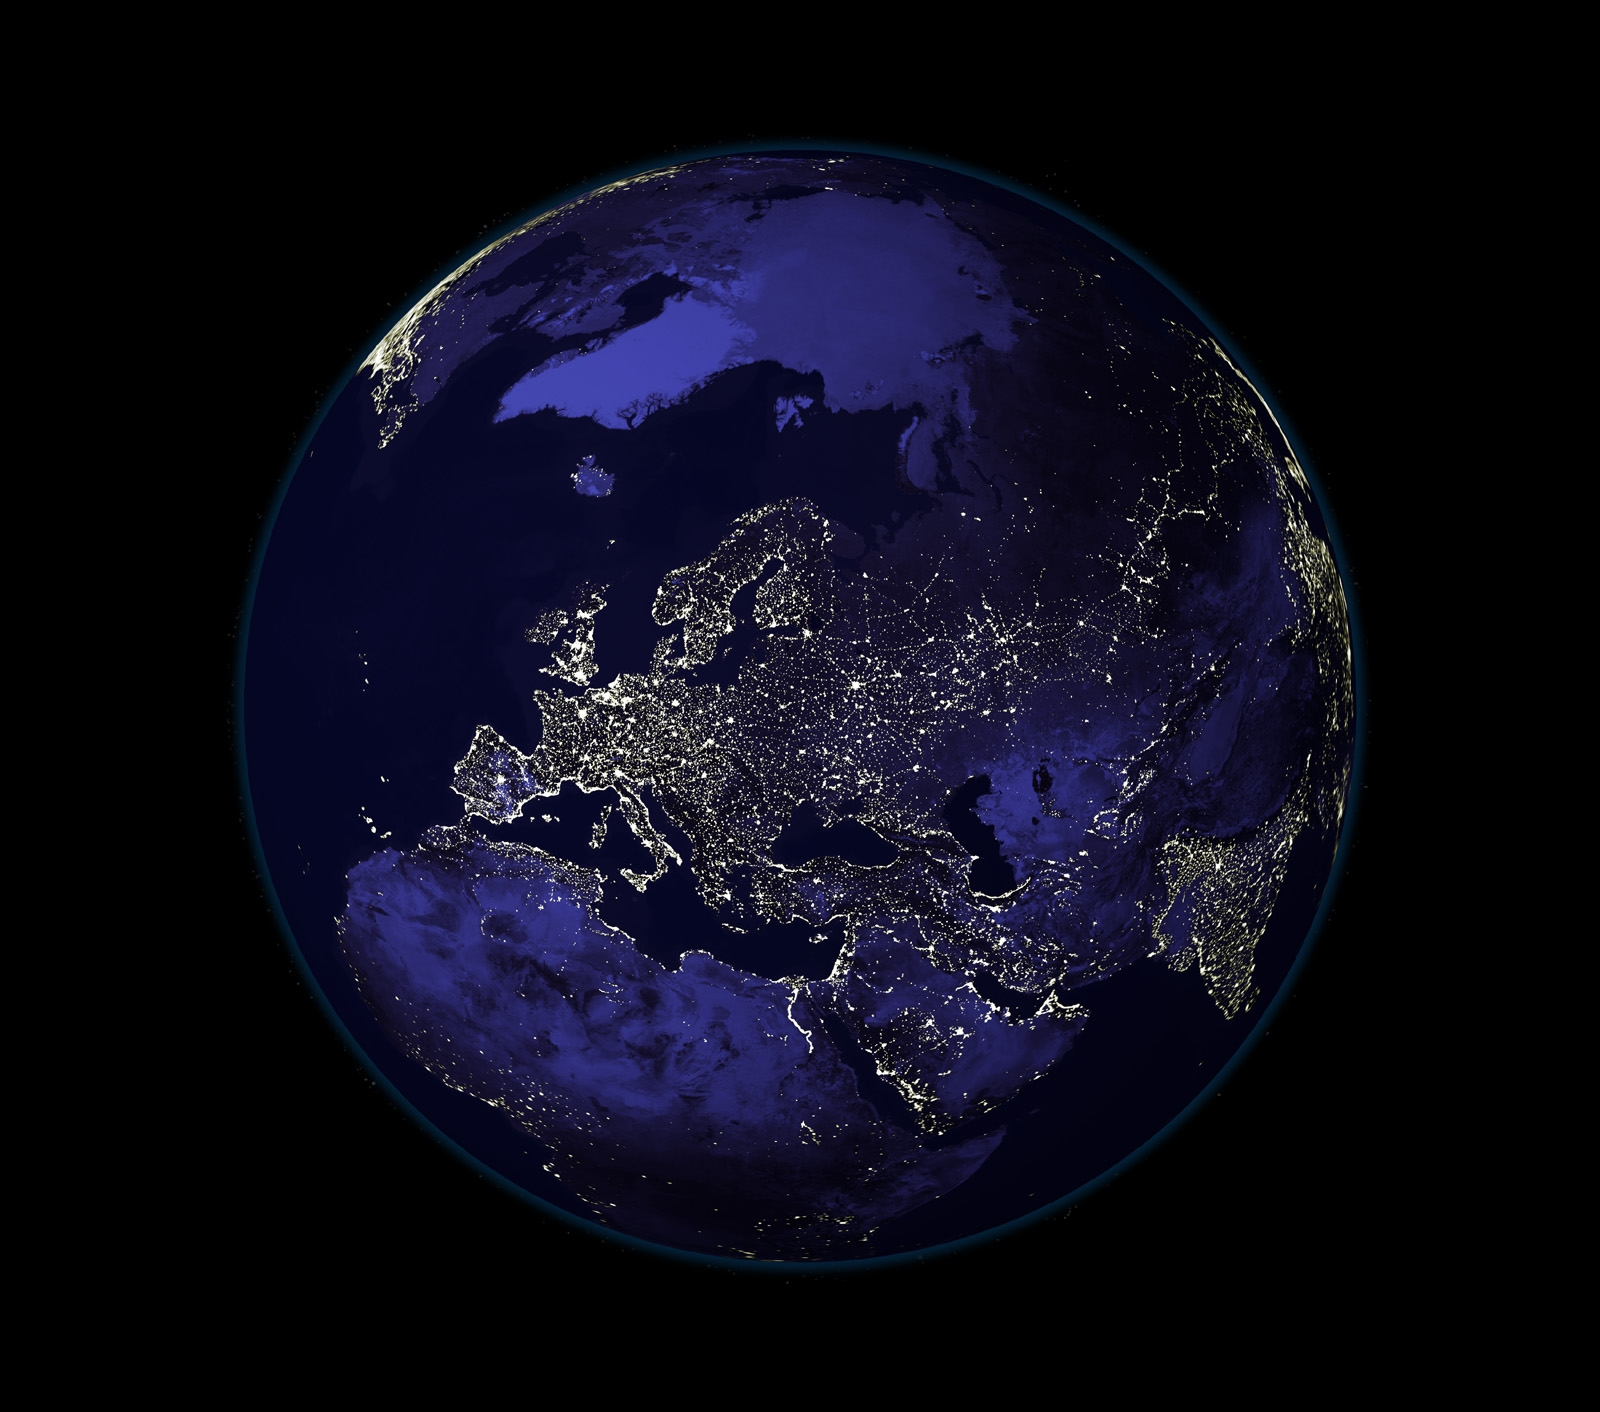
\includegraphics[width=\textwidth]{Tellus}
	\end{subfigure}
	\begin{subfigure}[b]{0.3\textwidth}
		\caption{Spectrum of an earth twin}\label{fig:spectrum:earth:twin}
		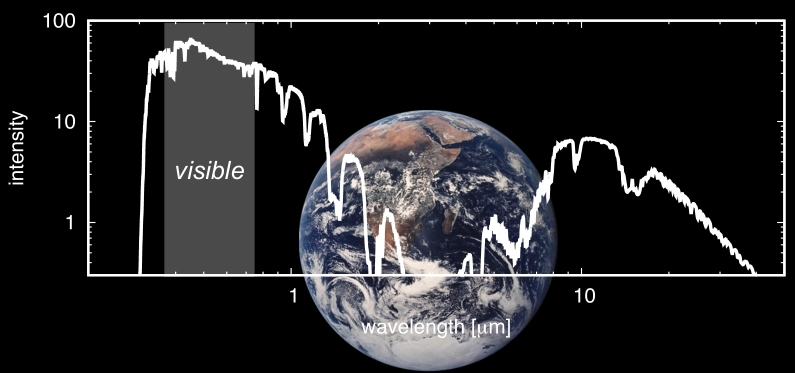
\includegraphics[width=\textwidth]{SpectrumEarthTwin}
	\end{subfigure}
	\begin{subfigure}[b]{0.3\textwidth}
		\caption{At shorter wavelengths the planet scatters light}\label{fig:spectrum:earth:twin1}
		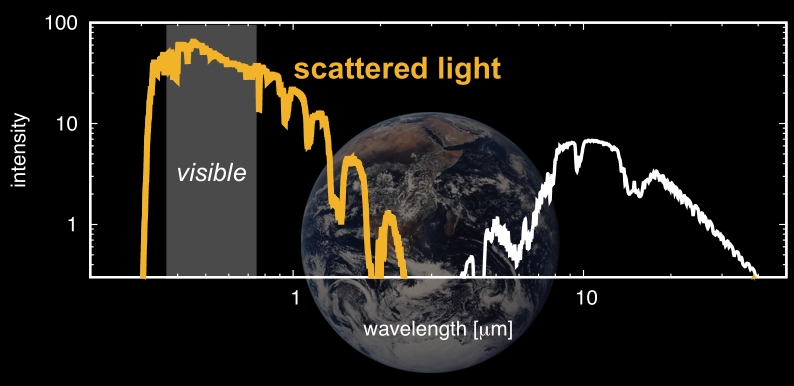
\includegraphics[width=\textwidth]{SpectrumEarthTwin1}
	\end{subfigure}
	\begin{subfigure}[b]{0.45\textwidth}
		\caption{At longer wavelengths it emits infrared}\label{fig:spectrum:earth:twin2}
		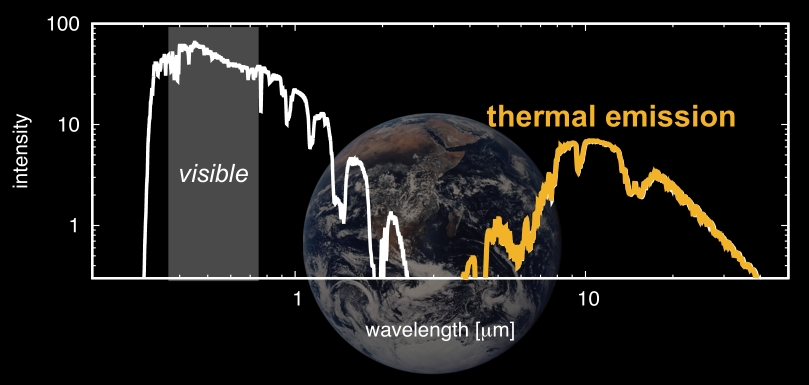
\includegraphics[width=\textwidth]{SpectrumEarthTwin2}
	\end{subfigure}
	\begin{subfigure}[b]{0.45\textwidth}
		\caption{Absorption by atmospheric species}\label{fig:spectrum:earth:twin3}
		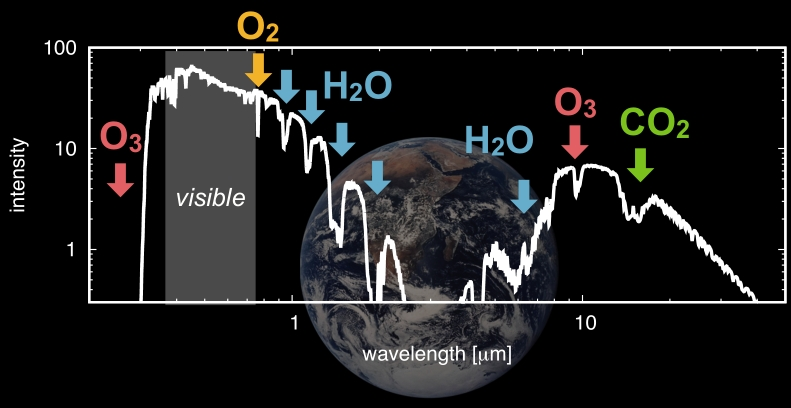
\includegraphics[width=\textwidth]{SpectrumEarthTwin3}
	\end{subfigure}
\end{figure}


At shorter wavelength,
the planet illuminates
by scattering the light
from the host star--Figure \ref{fig:spectrum:earth:twin1}.
And, it's blue features depend on,
for example,
surface composition,
atmospheric pressures and clouds.
On the other hand,
in the invisible infrared range,
the planet emits light
because of its thermal energy--Figure \ref{fig:spectrum:earth:twin2}--
and its baseline depends on
the temperature structure
of the surface layers.
Imprinted in these baselines
are the lower features
due to absorption
by atmospheric species--Figure \ref{fig:spectrum:earth:twin3}.
In the case of an Earth Twin,
they include astrobiologically important
water vapor, oxygen
and ozone features.

We could also potentially use
the time variation of these features
due to planet rotation,
which essentially allows us
to scan the planet
and highlight the regional features.
However, it's not straightforward
to detect the light from exoplanets.
Seen from afar, an exoplanet is
very close to its own host star,
and the star is several to ten
orders of magnitude brighter.
It's equivalent to seeing a firefly
right next to a lighthouse.
Suppose you try to take a picture
of an exoplanet.
Then, the host star is always there,
and, on the imaging plane,
the star is blurred
and the planet is in the skirt of it--Figure \ref{fig:StarIsMuchBrighter}.

\begin{figure}[H]
	\caption[The star is many orders of magnitude brighter than its planets]{Unfortunately the star is many orders of magnitude brighter than its planets}\label{fig:StarIsMuchBrighter}
	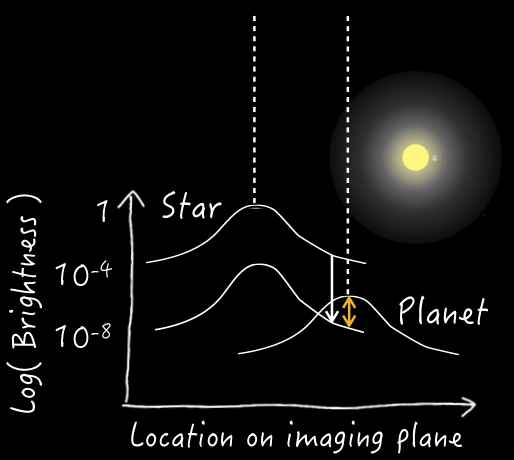
\includegraphics[width=\textwidth]{StarIsMuchBrighter}
\end{figure}

Compared to the peak intensity,
the skirt is orders of magnitude darker,
but planets are often even fainter,
so the signal is varied.
In order to identify the planetary signal,
we need to suppress the light
from the host star
using special instruments.
The idea of such direct imaging
observations of Earth-like planets
dates back to the 1990s.
But, the starlight suppression
is technically challenging.

In the past decade,
direct imaging has been successful
for young, luminous, giant,
gaseous planets at wide orbits--Figure \ref{fig:young:jupiter0}.
Earth-like planets are about
ten times smaller in diameter
and much fainter than
these successful targets.
The efforts are ongoing to achieve
the hyper-suppression level
to be able to detect an Earth Twin.


\begin{figure}[H]
	\caption{Success with Young Jupiter-like Planets in Distant Orbits}\label{fig:young:jupiter}
	\begin{subfigure}[b]{0.25\textwidth}
		\caption{Young Jupiter-like Planet}\label{fig:young:jupiter0}
		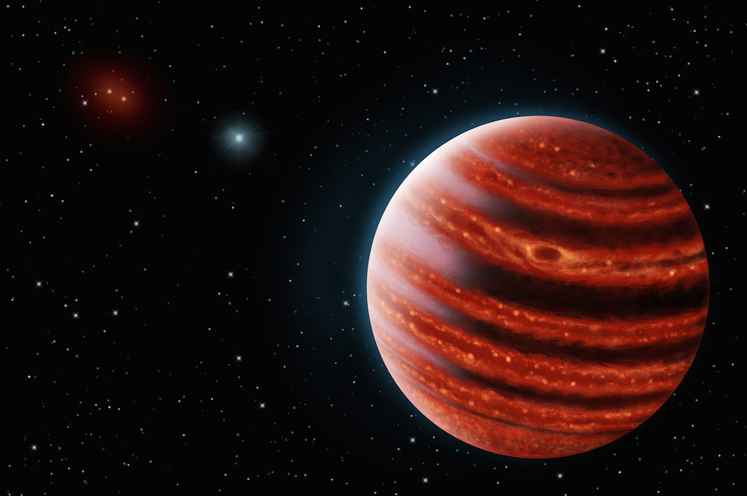
\includegraphics[width=\textwidth]{young-hot-jupiter}
	\end{subfigure}
	\;\;\;
	\begin{subfigure}[b]{0.3\textwidth}
		\caption{ Images of a fourth planet orbiting hr 8799\cite{marois2010images}}\label{fig:young:jupiter1}
		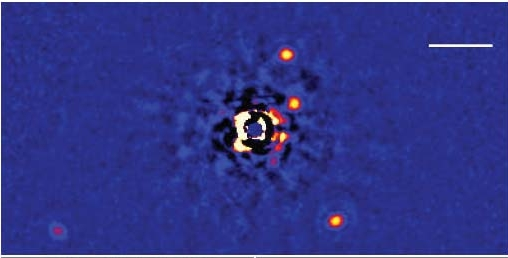
\includegraphics[width=\textwidth]{DirectImaging1.jpg}
	\end{subfigure}
	\;\;\;
	\begin{subfigure}[b]{0.35\textwidth}
		\caption{Gpi spectra of hr 8799 c, d,
			and e\cite{greenbaum2018gpi}}\label{fig:young:jupiter2}
		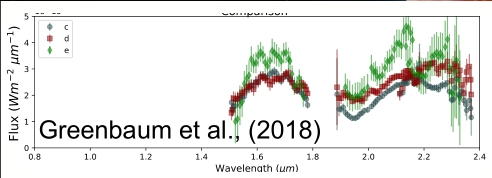
\includegraphics[width=\textwidth]{DirectImaging2.jpg}
	\end{subfigure}
\end{figure}

Meanwhile, the discovery
of transiting planets
opened up new possibilities
to study exoplanet atmospheres
without using special instruments--Figure \ref{fig:transiting:planets}.

\begin{figure}[H]
	\caption[Transiting Planets]{The discovery
		of transiting planets
		opened up new possibilities
		to study exoplanet atmospheres
		without using special instruments}\label{fig:transiting:planets}
	\begin{subfigure}[b]{0.2\textwidth}
		\caption{A transiting planet}\label{fig:transiting:planets1}
		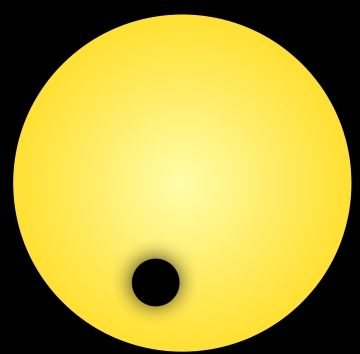
\includegraphics[width=\textwidth]{TransitingPlanets1}
	\end{subfigure}
	\;\;
	\begin{subfigure}[b]{0.3\textwidth}
		\caption{A planet which	passes right in front of the star
			because its orbital plane is close to the line of sight}\label{fig:transiting:planets2}
		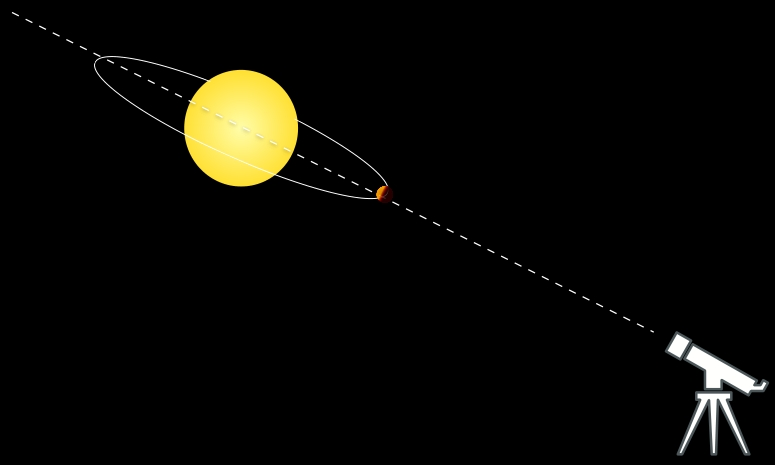
\includegraphics[width=\textwidth]{TransitingPlanets2}
	\end{subfigure}
	\;\;
	\begin{subfigure}[b]{0.31\textwidth}
		\caption{During the transit, a small portion
			of the stellar light
			is filtered through
			the planetary atmosphere}\label{fig:transiting:planets3}
		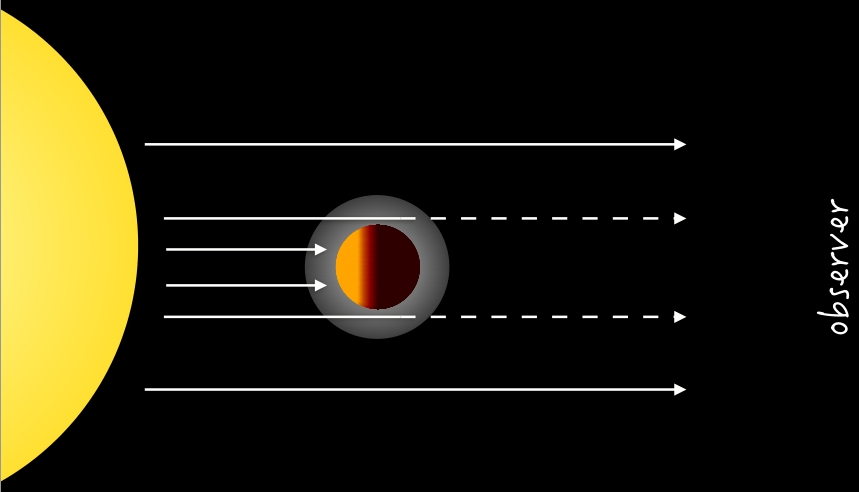
\includegraphics[width=\textwidth]{TransitingPlanets3}
	\end{subfigure}
\end{figure}

A transiting planet is a planet which
passes right in front of the star
because its orbital plane
is close to the line of sight--Figure \ref{fig:transiting:planets2}.
During the transit, a small portion
of the stellar light
is filtered through
the planetary atmosphere--Figure \ref{fig:transiting:planets3}.
By analyzing the spectrum
of this tiny portion
and finding the scattering
or absorption features in there,
we can learn about
the atmospheric composition
and the presence of condensates
such as clouds.
This technique is called
"transmission spectroscopy."

In many cases, transiting planets also pass behind the host star
and that's called "planetary" or "secondary" eclipse--Figure \ref{fig:secondary-eclipse}
\begin{figure}[H]
	\caption{Secondary Eclipse}
	\begin{subfigure}[b]{0.45\textwidth}
		\caption{In many cases, transiting planets also pass behind the host star
			and that's called "planetary" or "secondary" eclipse}\label{fig:secondary-eclipse}
		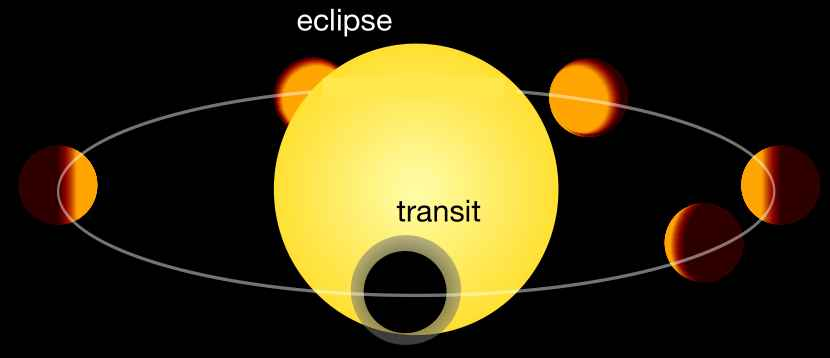
\includegraphics[width=\textwidth]{secondary-eclipse}
	\end{subfigure}
	\begin{subfigure}[b]{0.45\textwidth}
		\caption{The difference between
			the out-of-eclipse total flux
			and the in-eclipse flux
			corresponds to the brightness
			of the planetary dayside}\label{fig:secondary-eclipse1}
		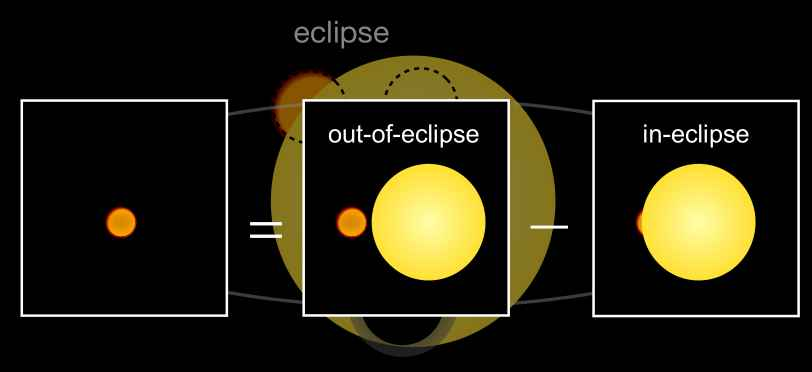
\includegraphics[width=\textwidth]{secondary-eclipse1}
	\end{subfigure}
\end{figure}
At the time of the eclipse,
the planetary flux is blocked by the star.
So, the difference between
the out-of-eclipse total flux
and the in-eclipse flux
corresponds to the brightness
of the planetary dayside--Figure \ref{fig:secondary-eclipse1}.
This way, using planetary eclipse,
we can identify the spectrum
of the planet
without directly separating the star
and the planet in the imaging plate.

In addition, while the planet
orbits the star,
the varying portion of the planetary
dayside faces us
and the planetary flux
changes in time accordingly--Figure \ref{fig:phase-variation}.

\begin{figure}[H]
	\begin{center}
		\caption[Phase Variation]{ while the planet orbits the star, the varying portion of the planetary dayside faces us 	and the planetary flux changes in time accordingly}\label{fig:phase-variation}
		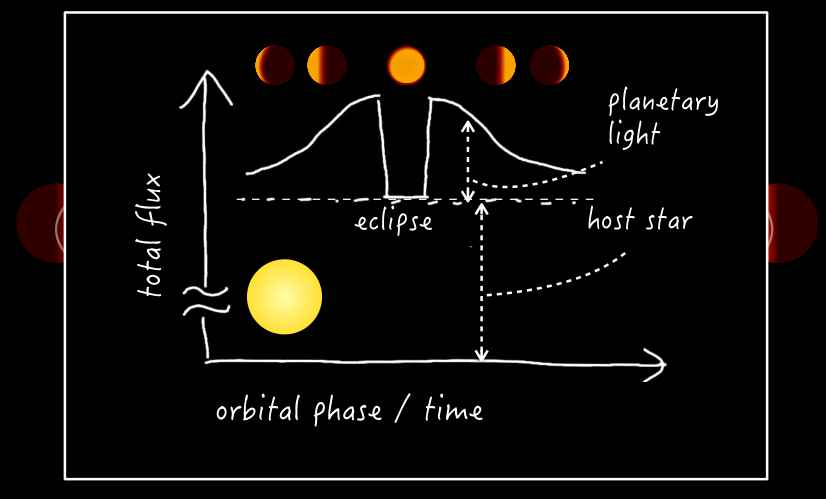
\includegraphics[width=0.8\textwidth]{phase-variation}
	\end{center}
\end{figure}
In turn, although we cannot resolve
the star and the planet,
the time variation in the total flux
can be attributed to
the planetary component
assuming that the star is stable.
These three techniques
have been successful
with hot Jupiter-like planets
and have revealed
some of the atmospheric species
and thermal structures.

In order to apply them to smaller,
potentially habitable planets, however,
we need to push the current
technology to its limit.
The techniques introduced so far
have pros and cons
and the relevant targets vary.
So, we will use all of them
to study various aspects of exoplanets.
In the next decade,
new powerful observatories
with spectroscopic capability
will come into play.
The main targets will probably be
large gaseous planets
but some basic investigations
of terrestrial sized planets
are also being attempted.
Future missions aimed at
the most detailed study
of potentially habitable planets
are currently under discussion.

In this lecture,
we discussed the key observations
to study the nature of exoplanets
beyond their size in the orbit.
I encourage you to think further
about how you would find life
on an Earth Twin light-years away
using these techniques.
It will provide and unique view
on Earth's biosphere.

Summary: Key observations to characterize atmospheres (and surfaces) of exoplanets
\begin{itemize}
	\item Direct Imaging
	\item  Transmission spectroscopy
	\item  Secondary eclipse
	\item  Phase curves
\end{itemize}
Using these techniques, how would you find life on an Earth-twin?


Here are some suggestions for further reading.

\cite{fujii2018exoplanet,sagan1993search,kaltenegger2017characterize,robinson2011earth,deming2013infrared,knutson2007map}

\section[Abstract and general Models for Life]{Abstract and general Models for Life--Sara Imari Walker}

One of the critical questions of
astrobiology is how do we model life and
we can think about abstract or general
models for life. The reason that we're
after those is because we want to not
only explain life on earth but we want
to be able to explain life on other
worlds and so we need to come up with as
general a principle as possible. So far a
lot of astrobiology has focused on the
idea of trying to define life, so we have
come up with a lot of different
definitions for life
from numerous different perspectives and
this word cloud--Figure \ref{fig:life-word-cloud} is just showing some
examples, words,
definitions for life and there are so
many different definitions for life that
has really become quite a muddle as to
how we should be thinking about it in a
more rigorous way.

\begin{figure}[H]
	\caption[Life from numerous different perspectives]{Life from numerous different perspectives\cite{trifonov2011vocabulary}}\label{fig:life-word-cloud}
	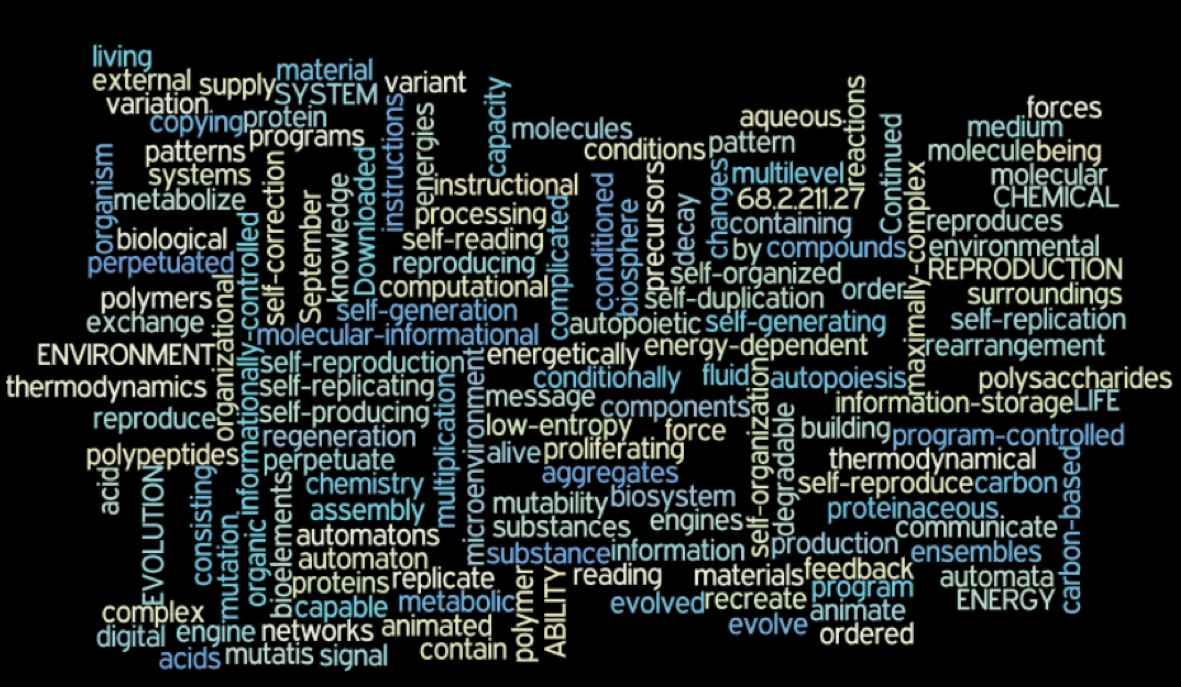
\includegraphics[width=\textwidth]{life-word-cloud}
\end{figure}

One of the things that  you think about as
an astrobiologist is: what's the
value of a definition versus a theory or
model. A lot of the traditional
literature and origins of life has been
focused on this idea of defining life so
that we can actually be able to identify
life on other worlds. The definitions
for life are really rather ad-hoc and in
some sense they're  from
observations of life on Earth:
\begin{itemize}
	\item  for example we know that life on Earth evolved so we might have an evolutionary definition of life;
	\item or we know that life on Earth is cellular so we might assume that all life requires cells.
\end{itemize}

What we ultimately really need to be aiming for
in the field of astrobiology is to build
better models and theories which might
be more general and allow us to move
beyond definitions of life that are
anthropocentric to our own life but
actually become predictive theories for
how life might look on other worlds.

The challenge that we face with anything
trying to get beyond an anthropocentric
or human-centered or earth-centered
viewpoint is that we only have a single
example of life on Earth; despite all
the diversity of life forms that we see
trees cats people bacteria in your gut
all of that life is related by a common
ancestry
and the way that astrobiologists talk
about that is to talk about
something called the \gls{gls:LUCA},
so if we look at the tree of life
as shown here--Figure \ref{fig:yatol}--and we trace
the evolution of all the life-forms that
exist today backwards in time they all
converge on what's called this \gls{gls:LUCA}, which is a
population of cells that lived on the
primitive earth.


\begin{figure}[H]
	\caption{We are limited by a single example of life}\label{fig:yatol}
	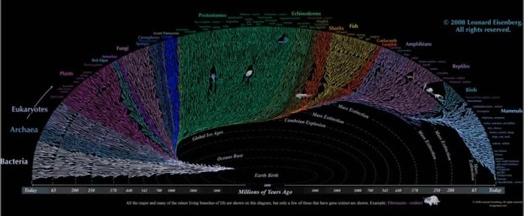
\includegraphics[width=\textwidth]{YATOL}
\end{figure}

We think that all
modern life descended from \gls{gls:LUCA}, and the
properties that that life-form would
have had would have had to have DNA and
a translation machinery proteins and
cellular architecture much like a modern
cell so it was actually a very advanced
life-form it doesn't take us all the way
back to the origins of life on earth but
the fact that all life shares is kind of
common biochemical architecture is
actually really limiting because it
means that we only have one example of
life to go on and extrapolating any kind
of general principles from one example
is actually rather hard.

What people have done traditionally in the origin of
life field is to try to come up with
models that are based on sort of the core
components of that architecture of life
that we know today and two of those core
components that have been dominant
models for origins of life are what are
called genetics first  metabolism first--Figure \ref{fig:GeneticsVsMetabolism}.

\begin{figure}[H]
	\caption[Genetics-First versus Metabolism-First]{Genetics-First versus Metabolism-First: Two competing hypotheses}\label{fig:GeneticsVsMetabolism}
	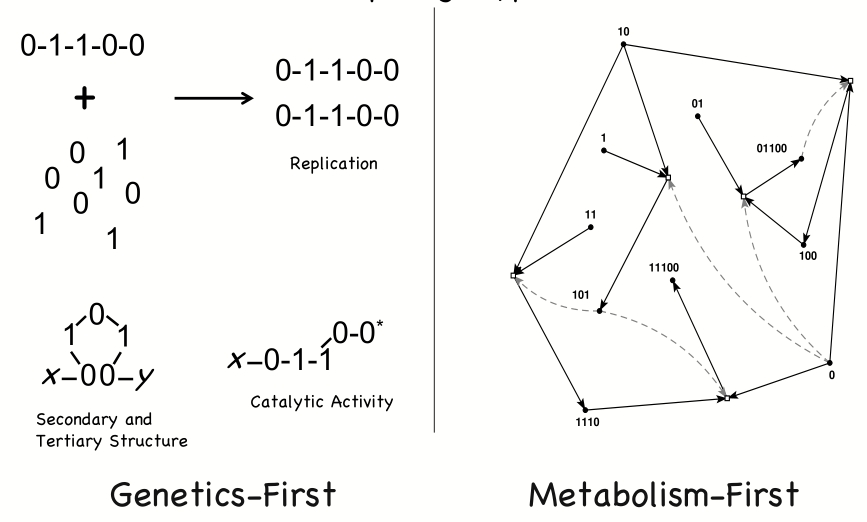
\includegraphics[width=0.9\textwidth]{GeneticsVsMetabolism}
\end{figure}

We know that cells metabolize
they need to acquire food from their
environment or you or I need to acquire
food in order to survive in order to
reproduce so metabolism is obviously a
critical component and then in the
genetics first view we also know that
life requires genetic information in
order to be able to reproduce and to
evolve over many generations and so if
you split these two kinds of core
components of biology and to just what
that essential thing is we have this
sort of genetics idea where people have
proposed that the first living entities
might have just been molecules like RNA
that could copy themselves and here on
the slide is shown sort of an
abstract model that kind of process
where you might just talk about the the
binary digits in a sequence if it was an
RNA molecule it would be the sequence of
ribonucleotides in the actual RNA so
that actual basis and you can actually
talk about reproducing that information
via copying and then the reason that the
RNA world
has been so popular as an idea is that
RNA also has a catalytic function
associated with it whereas in modern
organisms we have DNA and protein and
DNA controls genetic heredity and
proteins are primarily the catalysts
that actually execute reactions in the
cell, RNA can do both those functions so
genetics first has emerged of this idea
that you can model quite simply with
these kind of models where you talk
about copying and heredity and this idea
of evolution through this kind of
process as the core thing that emerged
first as a first living entity.

The metabolism first perspective is an
alternative view that the first kinds of
living entities were not individual
molecules that could replicate but sets
of molecules that were reacting together
and could collectively reproduce due to
the organizational patterns of their
reactions, and that idea is called
autocatalytic set theory and there's an
example shown here about a catalytic
sets, using that same kind of
representation of representing molecules
as binary strings, just strings of zeros
and ones which is a way of modeling
these kinds of processes in artificial
chemistries. And so in this metabolism-
first view the first kinds of living
systems would have been these organized
patterns of chemical reactions.

 And so
both of these perspectives allow one to
model certain attributes of living
systems. But it's really nice if you
actually put them side-by-side and look
at something like the binary polymer
representation of them because you start
to see that both of them are different
ways of propagating information in
chemical systems, and a theme starts to
emerge about what kinds of theories
might unify different approaches to
origins of life. And so this gets back to
the idea that what we need to start
doing to move forward in origins of life
whereas traditionally we've had these
models like genetics first, metabolism
first, and there's other models like
compartment first, where
we're talking about
mineral surfaces and all kinds of
things and that we need to really start
thinking about what are the theories for
life, and how do we actually develop more
predictive models that are more generic
too different chemistries and allow us
to actually go to the lab and predict
under what circumstances we should start
getting things that look more lifelike.

And a nice example of the need for
theories and thinking about origins of
life was given by Carol Cleland and
Chris Chyba and a paper that they wrote on
defining life where they talked about
trying to define water and how difficult
it was to actually define water before
we had a molecular theory for water so
you might describe water as a clear
liquid, you might describe it based on
the fact that it's liquid at a certain
range of temperatures that it you know
doesn't have a strong odor there's a lot
of different ways that you could
describe what water that might lead to a
definition of water but none of them are
really exclusive to water because
there's other clear liquids that you
might describe there's other things that
are also a liquid at room temperature
and so the way that we really precisely
define what water is is actually to have
an atomic theory that describes
molecules and their interactions and we
can precisely define water now as h2o
and so their thought was that what we do
now is sort of phemenologically define
life, we have a lot of heuristics or a
lot of ideas about what we think life
might be but ultimately what we need is
a theory and that our definition should
derive from the theory not the other way
around.

And one way I like to think about
that is actually to think about like the
emergent properties of life
so water for example,
one of the defining properties
that we think water has is that it's wet
but wetness of water is an emergent
property it requires many many many
millions of water molecules potentially
to be wet although there's
actually an active debate
about how many water molecules
if it's a few hundred a few
thousand and people have been working to
develop models to quantify when water
gets wet
likewise if we're thinking about
emergent properties of life evolution is
often considered to be a defining
property of life but evolution exists at
the level of population so it requires
many interacting individuals
in order to be an evolutionary
system and so in some sense evolution
that we use as a defining property of
life is also an emergent property of
life and so one of the things that we
really need to challenge ourselves with
is to try to find the underlying theory
that explains that emergent property in
the same way that we have an atomic
theory for water that explains some of
its emergent properties
and so one of
the ways that we might think about that
is actually to think about life as an
information processing system--Figure \ref{fig:nurse-information}.

\begin{figure}[H]
	\begin{center}
		\caption[Life as an information processing system]{Life as an information processing system\cite{nurse2008life}}\label{fig:nurse-information}
		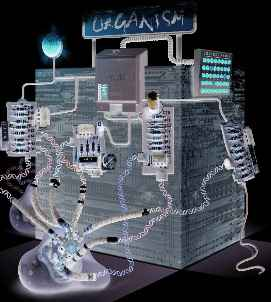
\includegraphics[width=0.6\textwidth]{nurse-information}
	\end{center}
\end{figure}




This is kind of a newer proposal about trying to
unify different properties of life that
a lot of people have been very
enthusiastic about in the field
and a lot of people are working on from
different perspectives but if we go back
to thinking about that genetics versus
metabolism picture
and we had the binary polymer model.
Both of those were kind of
a representation of an informational
system that was capable of reproducing
itself they were just very different
architectures for that kind of thing and
one might think of genetics first as a
digital type of information processing
and metabolism first as an analogue type
of information processing and so so
there is this idea in the biological
community and also emerging in
astrobiology about information possibly
being a unifying principle for how we
should think about life across all
scales and that may be organisms are
really organized by flows of information
so one way to think about the origin of
life potentially as kind of a new
perspective is to think about it as a
transition and how information is stored
propagated and used and this might be
sufficiently general to be able to
predict properties of alien chemistries
that can also process information in a
similar way potentially to Earth's
biology but might allow different
chemistries than that biochemical
architecture that we have on earth as
characteristic
of the last Universal common ancestor
--Figure \ref{fig:LifeInformation}.
\begin{quotation}
	Focusing on information… may perhaps provide our best shot at uncovering universal laws of life that work not just for biological systems with known chemistry but also for putative artificial and alien life--\cite{cronin2016beyond}.
\end{quotation}

\begin{figure}[H]
	\caption[Life as Information]{Life as Information\cite{cronin2016beyond}}\label{fig:LifeInformation}
	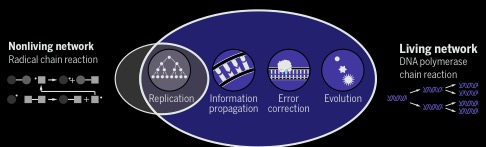
\includegraphics[width=0.9\textwidth]{LifeInformation}
\end{figure}


If we could
understand how information works in
biochemical networks on earth we could
potentially understand what other
possible chemistries could enable those
same kinds of emergent properties on
other worlds and maybe predict alien
chemistries

\section[The Multiple Origins of Life]{The Multiple Origins of Life--David Krakauer}


\subsection{The Argument}

\begin{itemize}
	\item Origin of Life Research is dominated by Naturalist-reductionists. \begin{quotation}
		My car and my adding machine 	understand nothing: they are not in that line of business--John Searle
	\end{quotation}

	\item an alternative would be Functionalists (like AI before Turing and modern ML)
	\begin{quotation}
		We are not interested in the fact that the brain has the consistency of cold porridge--Alan Turing.
	\end{quotation}

	\item Life emerges from an adaptive arrow of time (the reverse of the thermodynamic arrow).
	\item The Adaptive arrow of time is multi-scale and applies as readily to inference as organic evolution (this is not dependent on biological chemistry)
	\item The key to any form of adaptive evolution is the Agent, AKA, the Individual
	\item Individuals have evolved countless times in earth history - emerging from
	forms both ecological and individual: e.g. Virus evolution and the Block Chain.
\end{itemize}

\subsection{Reversing the Arrow of Time}

\begin{itemize}
	\item[Thermodynamic arrow] ''Let us draw an arrow arbitrarily. If as we follow the arrow we find more and more
	of the random element in the state of the world, then the arrow is pointing towards
	the future; if the random element decreases the arrow points towards the past … I
	shall use the phrase “time's arrow” to express this one-way property of time which
	has no analogue in space''--Arthur Eddington\cite{eddington1939philosophy}
	
	\item[Adaptive arrow]''It was Darwin’s chief contribution, not only to Biology but to the whole of natural science, to have brought to light a process by which contingencies a priori
	improbable are given, in the process of time, an increasing probability, until it is their non-occurrence, rather than their occurrence, which becomes highly improbable.''--Ronald Fisher\cite{fisher1930genetical}
\end{itemize}

\begin{figure}[H]
	\caption[Thermodynamic Arrow of Time versus Adaptive ]{Thermodynamic Arrow of Time wants to roll down hill, Adaptive up hill towards lower probability.}\label{fig:NaturalSelection}
	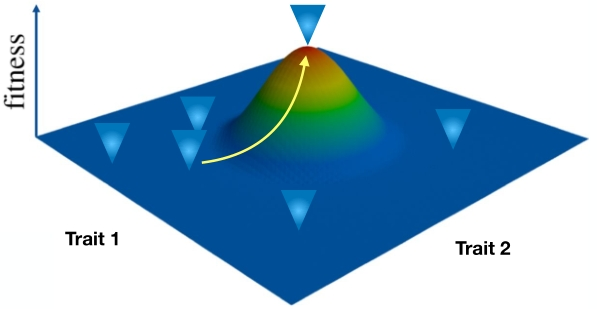
\includegraphics[width=0.9\textwidth]{NaturalSelection}
\end{figure}

\subsection{The Theory of the Adaptive Arrow of Time}

\begin{itemize}
	\item The Fundamental Theorem of Natural Selection
	R.A. Fisher, 1930
	\item ''adaptation is an optimization dynamics
	transferring information
	from the environment into the agent
	- reducing uncertainty about states of the world''\cite{rockmore2018cultural}
	\item A scale-invariant, substrate-neutral, stochastic process
	\begin{itemize}
		\item Evolution
		\item Inference
		\item Learning
	\end{itemize}
\end{itemize}

\subsection{Evolutionary Agents}

Sol Spiegelman wanted to know what was the minimal genome for \textit{Q Beta Phage}. He bred 74 generations in the presence of \textit{QBeta RNA replicase}, which it would normally have to synthesize--Figure \ref{fig:SpiegelmanMonster}. The RNA reduces from 4500 base pairs to 218!\cite{spiegelman1965synthesis}
\begin{figure}[H]
	\caption{The Spiegelman Monster}\label{fig:SpiegelmanMonster}
	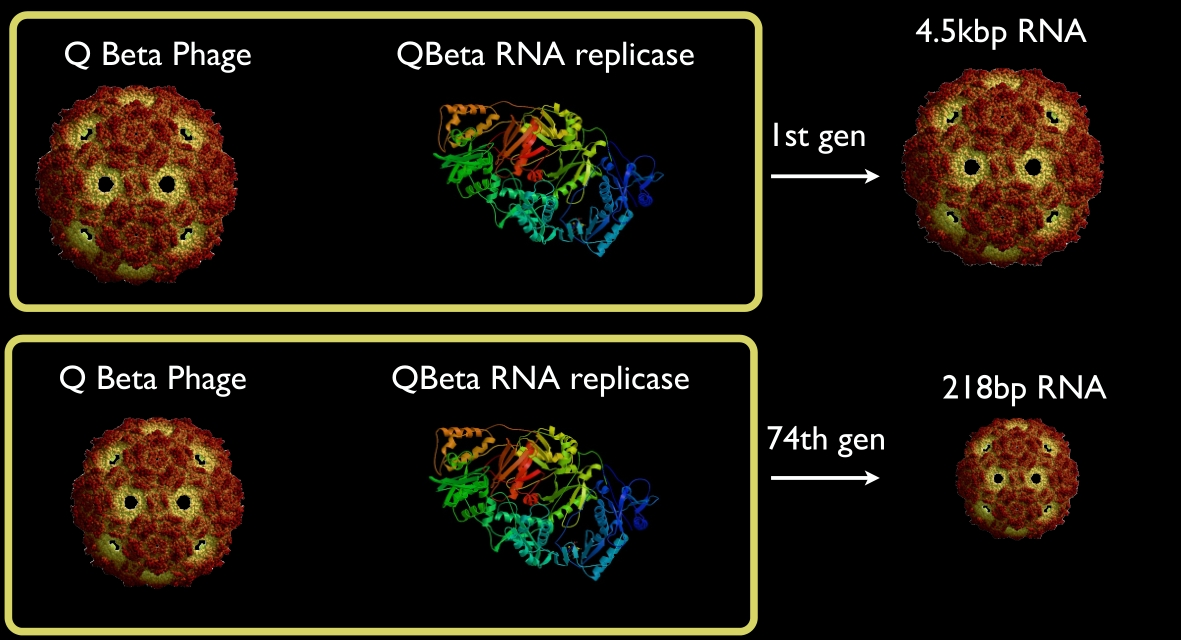
\includegraphics[width=0.9\textwidth]{SpiegelmanMonster}
\end{figure}

Figure \ref{fig:SpiegelmanMonsterVenn} depicts the process: $v_i$ represents the information held by the virus only, $h_i$ the information held by the host (environment), and $s_i$ the information that is shared. The virus eliminates the shared information if the information is always there! If we don't know that the information is always there, we get autonomy.

\begin{figure}[H]
	\caption{Elimination of shared Information}\label{fig:SpiegelmanMonsterVenn}
	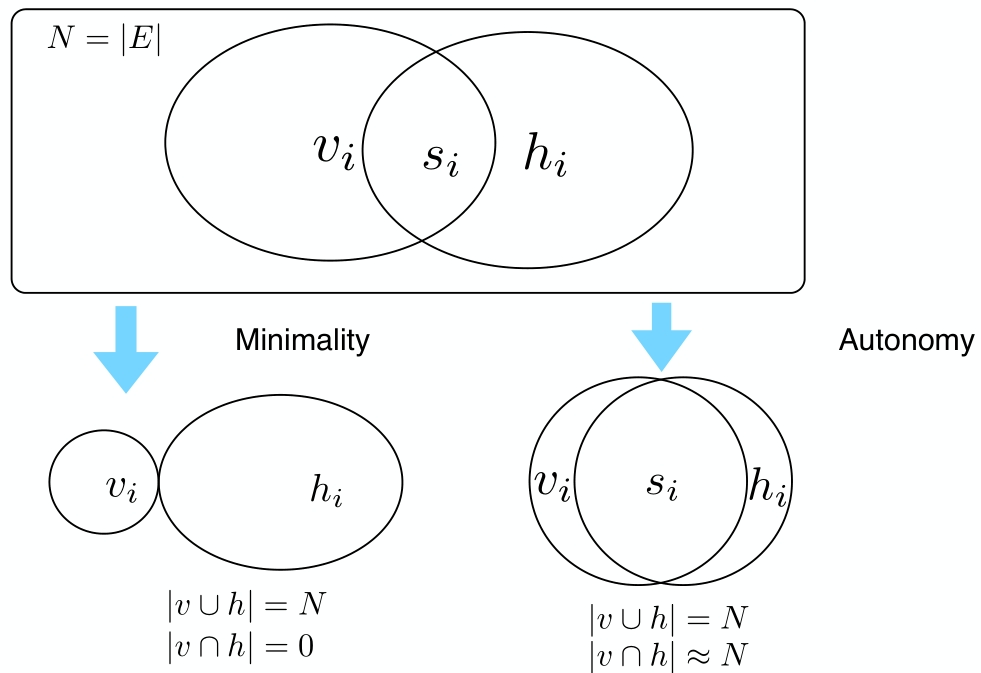
\includegraphics[width=0.9\textwidth]{SpiegelmanMonsterVenn}
\end{figure}

 Virus is normally considered as non-living, because it depends its environment, but we depend on our environment too, e.g. for vitamins. There is a spectrum of adaptive agency--Figure \ref{fig:SpectrumOfLife}.  ''Life is a mechanism for acquiring adaptive information about the World, that it propagates forward in time''. This includes computer viruses and blockchain!
 
\begin{figure}[H]
	\caption{The Spectrum of Life}\label{fig:SpectrumOfLife}
	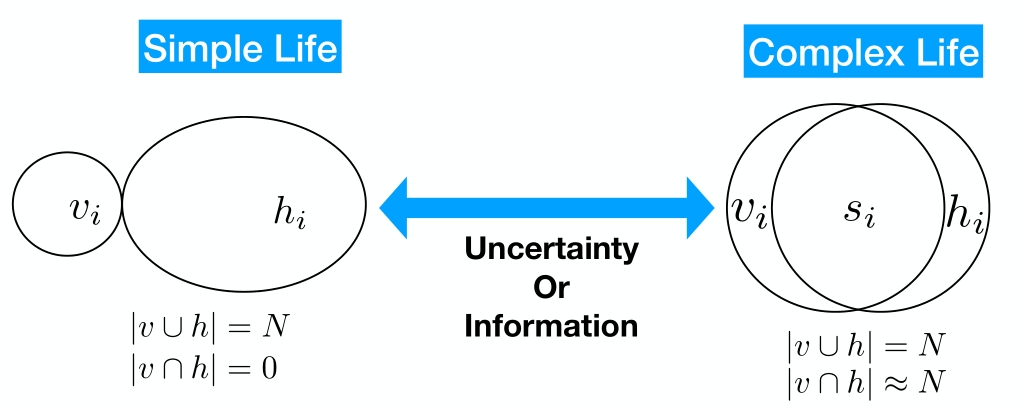
\includegraphics[width=0.9\textwidth]{SpectrumOfLife}
\end{figure}
Open Questions

\begin{itemize}
	\item[Fundamentalists] Are we only interested in the initial necessary conditions for all subsequent life (e.g. Evolveability out of abiotic physics as the most fundamental basis for understanding).
	\item[Pluralists] Or are we interested in the multiple origins of life (adaptive agency) and thereby the many analogous processes that can support these (e.g. 	Coarse-Grained effective theories at multiple scales?)
\end{itemize}


\section{Evolutionary Computation}

Lecturer: Stephanie Forrest

Evolution as computation.

Basic Principles of Evolution
\begin{itemize}
	\item Random variation
	\item Selection
	\item Inheritance
\end{itemize}

What are the genetic representations?
\begin{itemize}
	\item  Discrete units (genes)
	\item Genotype vs. phenotype
	\item Information stored in a linear array
\end{itemize}

Figure \ref{fig:GeneticAlgorithm} shows a Genetic Algorithm, as introduced by John Holland\cite{holland1992adaptation}, and Figure \ref{fig:GAfitness} shows a typical performance curve.

\begin{figure}
	\caption{Genetic Algorithm, exhibiting Selection, Crossover, and Mutation}\label{fig:GeneticAlgorithm}
	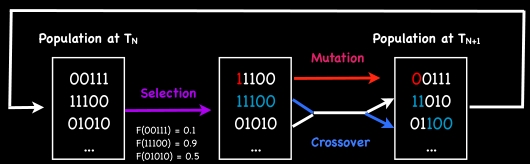
\includegraphics[width=0.9\textwidth]{GeneticAlgorithm}
\end{figure}

\begin{figure}
	\caption{Example Fitness Curve, with two plateaux}\label{fig:GAfitness}
	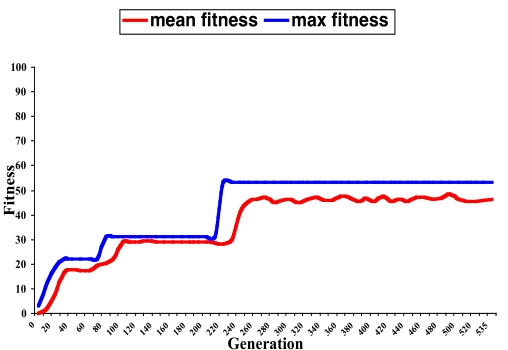
\includegraphics[width=0.9\textwidth]{GAfitness}
\end{figure}

Applications
\begin{itemize}
	\item  Engineering
	\begin{itemize}
		\item 	Multi-parameter function optimization\cite{marshall2014evolution}
	\end{itemize}
\end{itemize}

Origins of Evolutionary Computing

\begin{itemize}
	\item John Holland \cite{holland1992adaptation}
	\item Ingo Rechenberg \cite{rechenberg1965cybernetic}
	\item David Fogel et al\cite{fogel1998artificial}
	\item John Koza--evolving computer programs\cite{koza1992genetic}
\end{itemize}

See also \cite{mitchell1998introduction}, \cite{eiben2003introduction}, \cite{forrest1993genetic}, and \cite{ma2014novo}.



\section{Scaling}

Lecturer: Pablo Marquet

Why is scaling important?

\begin{itemize}
	\item Provides a way to deal with the diversity of scales and
	organisms found in ecological systems
	\item Makes apparent the fundamental similarity that
	underlies diversity in nature and how this has been
	molded by evolution
	\item Provides a benchmark against which species,
	populations and ecosystems can be compared
\end{itemize}

Many ecological attributes scale with size--(\ref{eq:PowerLawScaling}) and Figure \ref{fig:PowerLawScaling}.
\begin{align*}
	y \propto& M^{\alpha}\text{, where $M$ represents mass, size, etc.}\numberthis\label{eq:PowerLawScaling}\\
	=& c M^{\alpha}\\
	\implies&\\
	\log(y)=&\log(c) + \alpha \log(M)
\end{align*}

\begin{figure}[H]
	\caption{Many ecological attributes scale with size}\label{fig:PowerLawScaling}
	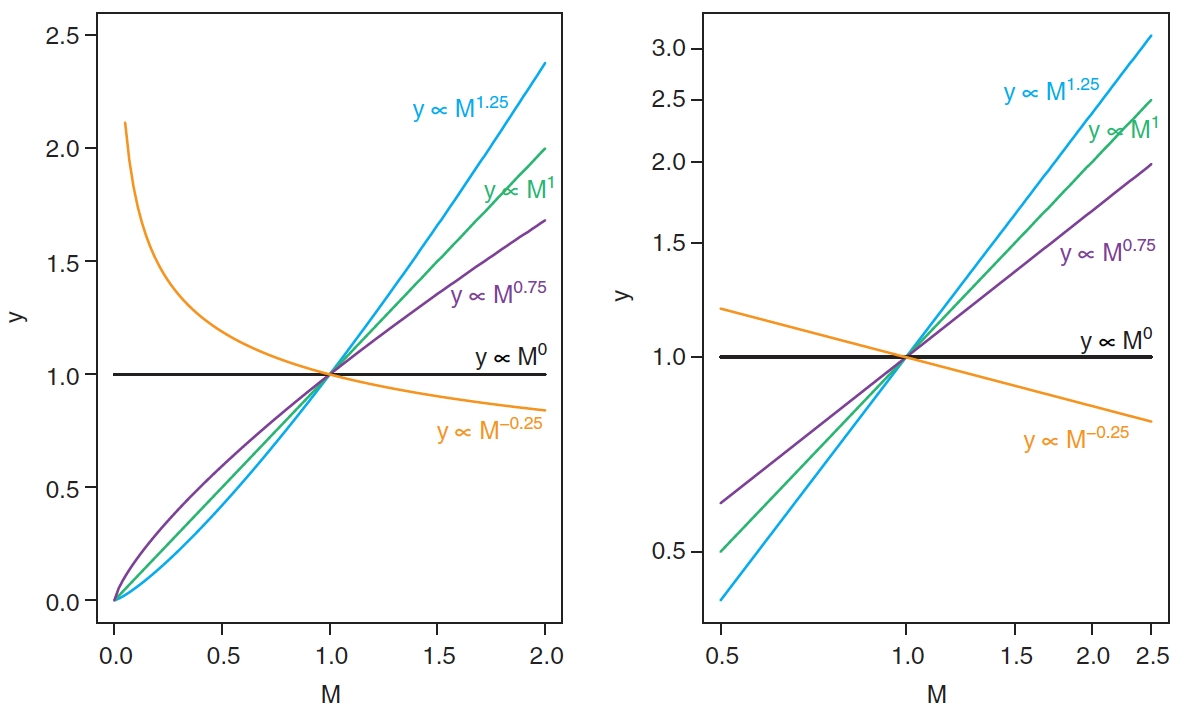
\includegraphics[width=0.9\textwidth]{PowerLawScaling}
\end{figure}

Figure \ref{fig:ScalingExamples} shows some examples, after \cite{sibly2012metabolic}. Mammals are in grey, marsupials in red. We can use this as a basis for investigating why mammals deviate.
\begin{figure}[H]
	\caption[Scaling of life-history events]{Scaling of life-history events: mammals are in grey, marsupials in red.}\label{fig:ScalingExamples}
	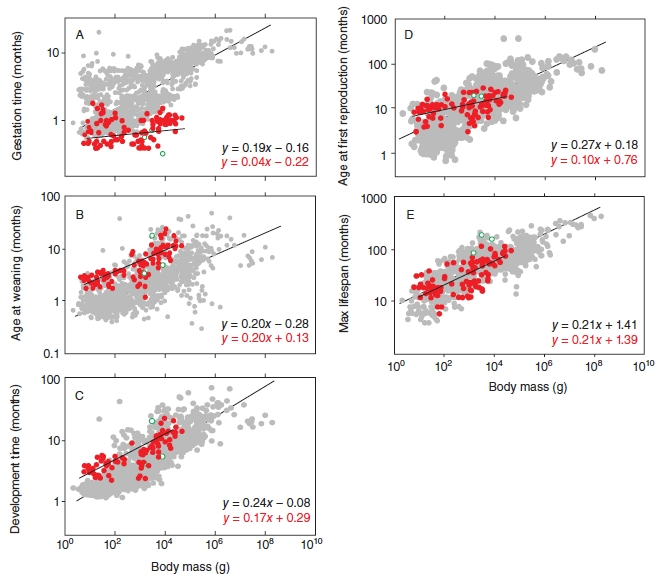
\includegraphics[width=0.9\textwidth]{ScalingExamples}
\end{figure}


Figure \ref{fig:Scaling:individuals:ecosystems}	depicts Mean Carnivore Mass-- Figure \ref{fig:mcm} \cite{tucker2014evolutionary}; Carbon Turnover--Figure \ref {fig:ct} \cite{anderson2013altered}; and Primary Production--Figure \ref{fig:npp} \cite{enquist2012land}.

\begin{figure}[H]
	\caption{Scaling in individuals and	ecosystems}\label{fig:Scaling:individuals:ecosystems}
	\begin{subfigure}[b]{0.45\textwidth}
		\caption{Mean Carnivore Mass}\label{fig:mcm}
		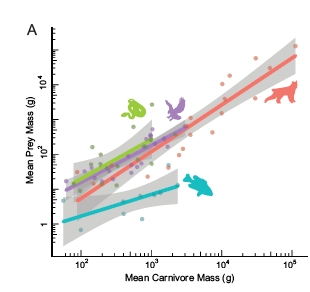
\includegraphics[width=\textwidth]{Scaling1}
	\end{subfigure}
	\begin{subfigure}[b]{0.45\textwidth}
		\caption{Carbon Turnover}\label{fig:ct}
		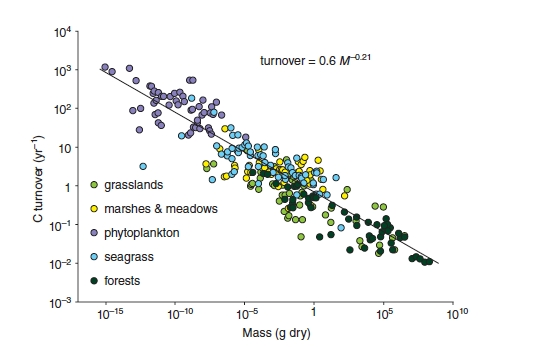
\includegraphics[width=\textwidth]{Scaling2}
	\end{subfigure}
	\begin{subfigure}[b]{0.45\textwidth}
		\caption{Primary Production}\label{fig:npp}
		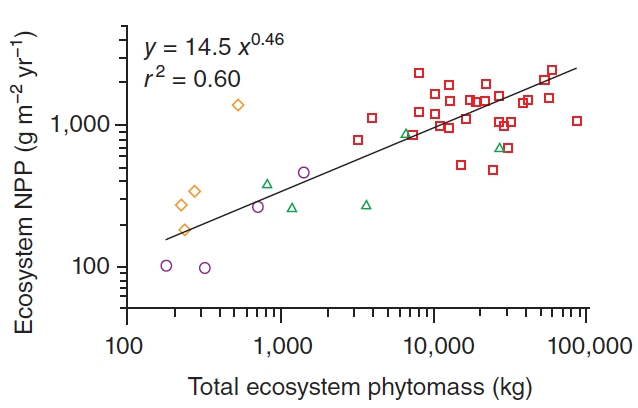
\includegraphics[width=\textwidth]{Scaling3}
	\end{subfigure}
\end{figure}

The central role of energy: the size ($M$) of an individual affects the amount
of energy it requires to maintain itself (basal metabolism $B$)--Figure \ref{fig:Kleiber} \cite{schmidt1984scaling}.

\begin{figure}[H]
	\caption{Kleiber's Law: $B \propto M^\frac{3}{4}$}\label{fig:Kleiber}
	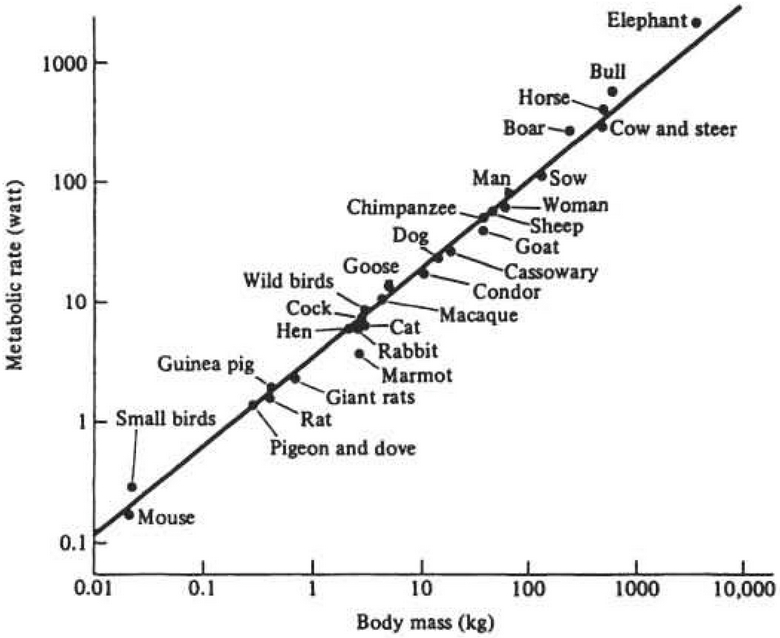
\includegraphics[width=0.9\textwidth]{Kleiber}
\end{figure}

Figure \ref{fig:Kleiber} suggest that somehow an elephant is just a large mouse! Natural Selection is not acting randomly, but is subject to constraints. The West, Brown \& Enquist developed a general model for the origin of allometric scaling laws in biology\cite{west1997general}.
\begin{itemize}
	\item The properties of resource delivery networks determine
	the properties of whole-organism metabolic rate.
	\item  Biological systems have evolved under natural
	selection to optimize performance (delivery networks
	minimize energy loss)
\end{itemize}

Some implications 

\begin{itemize}
	\item What is the maximum number of individuals that can be found in a given area--(\ref{eq:max}) and Figure \ref{fig:MammalianHerbivores} \cite{damuth1981population}?
	\begin{align*}
	R=& \text{Energy or resources per unit area}\\
	B=&\text{Individual resource requirements}\\
	N_{max}\propto& R M^{-\frac{3}{4}}\label{eq:max}\numberthis
	\end{align*}
	\begin{figure}[H]
		\caption{Mammalian Herbivores--$N_{max}\propto R M^{-\frac{3}{4}}$}\label{fig:MammalianHerbivores}
		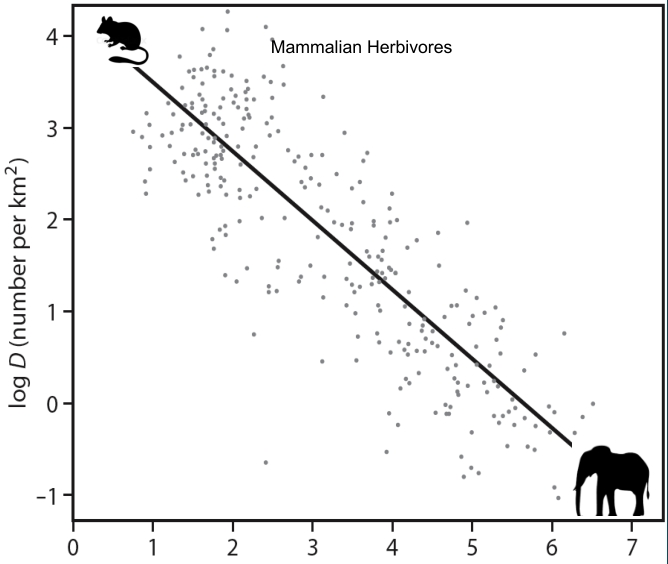
\includegraphics[width=0.9\textwidth]{MammalianHerbivores}
	\end{figure}	
	\item Populations of different organisms tend to use the same amount of energy--(\ref{eq:const}), Figure \ref{fig:PopulationEnergyUse} \cite{enquist1998allometric} 
	\begin{align*}
	E_{pop}\propto&N B\text{, Energy use for population}\\
	\propto& M^{-\frac{3}{4}} M^{\frac{3}{4}}\\
	\propto& 1\label{eq:const}\numberthis
	\end{align*}
	\begin{figure}[H]
		\caption{Population Energy Use}\label{fig:PopulationEnergyUse}
		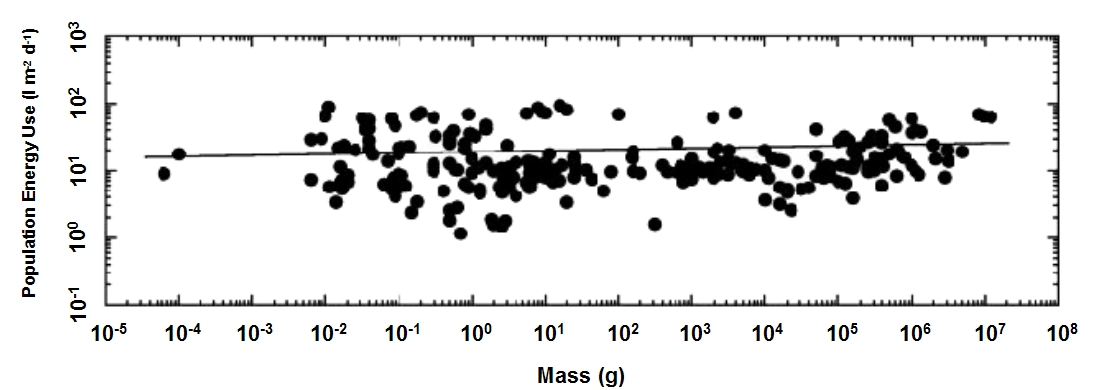
\includegraphics[width=0.9\textwidth]{PopulationEnergyUse}
	\end{figure}
	\item Humans--the hyper-dense species--Figure \ref{fig:Hyperdense}
	\begin{figure}[H]
		\caption{Humans--the hyper-dense species}\label{fig:Hyperdense}
		\includegraphics[width=0.9\textwidth]{Hyperdense}
	\end{figure}
\end{itemize}

See also \cite{marquet2005scaling}

\section{Energy}

Lecturer: Van Savage

How is energy used in biology?

\begin{itemize}
	\item Used for infinitely many things
	\item Art of science is drawing boxes in useful ways
	\item What main boxes of energy do we need to consider for evolution and	ecological systems?
	\begin{itemize}
		\item Development/Growth
		\item Maintenance
		\item Reproduction
	\end{itemize}
	\item How do organisms obtain and produce energy?
	\begin{itemize}
		\item Obtaining resources
		\item Processing energy
		\item Distributing energy
		\item Converting energy (mitochondria)
	\end{itemize}
\end{itemize}

Metabolic rate depends on optimized networks and body size--Figure \ref {fig:MammalianBasalMetabolicRate} \cite{savage2004predominance}.

\begin{figure}[H]
	\caption{Metabolic rate depends on optimized networks and body size}\label{fig:MammalianBasalMetabolicRate}
	\begin{subfigure}[p]{0.45\textwidth}
		\caption{Mammalian Basal Metabolic Rate}
		\includegraphics[width=0.9\textwidth]{MammalianBasalMetabolicRate}
	\end{subfigure}
	\begin{subfigure}[p]{0.45\textwidth}
		\caption{Whole Plant Xylum Flux}
		\includegraphics[width=0.9\textwidth]{WholePlantXylumFlux}
	\end{subfigure}
\end{figure}

Metabolic rate depends on body temperature--Figure \ref{fig:BodyTemperature} \cite{dell2011systematic}.

\begin{figure}[H]
	\caption{Metabolic rate depends on body temperature}\label{fig:BodyTemperature}
	\includegraphics[width=0.9\textwidth]{BodyTemperature}
\end{figure}

Affects all physiology--Figure \ref{fig:MammalianRestingHeartRate}\cite{savage2004predominance}.

\begin{figure}[H]
	\caption{Mammalian Resting Heart Rate}\label{fig:MammalianRestingHeartRate}
	\includegraphics[width=0.9\textwidth]{MammalianRestingHeartRate}
\end{figure}

And Ecology--Figure \ref{eq:AndEcology} \cite{ernest2003thermodynamic}.

\begin{figure}[H]
	\caption{And Ecology}\label{eq:AndEcology}
	\begin{subfigure}[b]{0.5\textwidth}
		\caption{Temperature Corrected Individual Production}
		\includegraphics[width=\textwidth]{AndEcology1}
	\end{subfigure}
	\begin{subfigure}[b]{0.5\textwidth}
		\caption{Temperature Corrected Population Density}
		\includegraphics[width=\textwidth]{AndEcology2}
	\end{subfigure}
\end{figure}
See also \cite{odum1976energy}, \cite{odum1983systems}, \cite{schmidt1997animal}, \cite{brown2004toward}, and \cite{kempes2017thermodynamic}.

\section{Nonequilibrium Physics}

Lecturer: Eric Smith, External Professor, Santa Fe Institute.\\
\\
Topics covered:
\begin{itemize}
	\item The equilibrium concept of phase transition
	
	\item How phase transitions explain robust patterns
	
	\item Why equilibrium isn’t enough to understand life
	\item Phase transitions in dynamical systems ''frozen motion''
\end{itemize}

The ''ordinary'' response of thermodynamic systems to controls. E.g. lava: Viscosity increases smoothly as temperature is lowered. Phase transitions are different
\begin{itemize}
	\item Water does not become harder as it is cooled
	\item It turns to ice suddenly (critical temperature)
	\item The average direction of pointing of the ice sharply increases from zero at the freezing temperature
	\item The direction and strength of the crystal is called the ''Order 	Parameter'' of the transition
	\item Change is sudden because ''you can’t have half a symmetry''
	\begin{itemize}
		\item A direction either exists or it doesn’t
		\item All frozen directions are equivalent
	\end{itemize}
	\item Phase transitions, cooperatively-maintained states, and robustness
	\begin{itemize}
		\item Diamonds are hard because many atoms lock each other in place
		\item The order of the crystal is a ''robust'' property of freezing
	\end{itemize}
\end{itemize}

Evolution happens on a background of robust architectures
\begin{itemize}
	\item Universal small metabolites
	\item RNA and proteins
	\item Cellular and genomic individuality
\end{itemize}

Equilibrium ideas are not enough to explain the robust order of life (Chicken vs. chicken soup)


The Miller-Urey synthesis of amino acids\cite{miller1959organic}

Life is made of interlocking structures and processes: can phase transition ideas
be applied to these?

What might be the order parameters of life?

\begin{itemize}
	\item They would be chemical and energetic
	\item They would involve interdependent	structure and process
\end{itemize}

The characteristic molecules
\begin{itemize}
	\item Unchanging universal roles 	for small metabolites
	\item Key macromolecules such as RNA
\end{itemize}

The great biogeochemical cycles
\begin{itemize}
	\item Life alters cycling of Carbon, Nitrogen, Sulfur, and more
	\item New compounds are also formed of 	these elements
\end{itemize}

\begin{figure}[H]
	\caption[The great biogeochemical cycles]{The great biogeochemical cycles\cite{falkowski2008microbial}}\label{fig:biogeochemical} 
	\includegraphics[width=0.9\textwidth]{biogeochemical}
\end{figure}



\begin{figure}[H]
	\caption[Earth’s energy throughput]{Earth’s energy throughput: the Biosphere changes the way a planet converts sunlight into heat.\cite{meadows2005modelling}}\label{fig:EnergyThroughput} 
	\includegraphics[width=0.9\textwidth]{EnergyThroughput}
\end{figure}

The emergences of individualities
\begin{itemize}
	\item Individuality takes many 	forms
	\item The order parameters in individual-based systems 	are proper names
\end{itemize}

Take-home messages from the lecture:
\begin{itemize}
	\item Phase transitions are one way natural systems  spontaneously form order
	\item The order is robust due to mutual reinforcement
	\item Phase transitions can also lead to spontaneous order in processes like fractures
	\item Candidates for living order parameters include chemical cycles and individuality
\end{itemize}




% end of text 

% glossary
\printglossaries

% bibliography go here
 
\bibliographystyle{unsrt}
\addcontentsline{toc}{section}{Bibliography}
\bibliography{origins,wikipedia}

\end{document}
